% Copyright (C) 2014-2020 by Thomas Auzinger <thomas@auzinger.name>

\documentclass[draft,final]{vutinfth} % Remove option 'final' to obtain debug information.

% Load packages to allow in- and output of non-ASCII characters.
\usepackage{lmodern}        % Use an extension of the original Computer Modern font to minimize the use of bitmapped letters.
\usepackage[T1]{fontenc}    % Determines font encoding of the output. Font packages have to be included before this line.
\usepackage[utf8]{inputenc} % Determines encoding of the input. All input files have to use UTF8 encoding.

% Extended LaTeX functionality is enables by including packages with \usepackage{...}.
\usepackage{amsmath}    % Extended typesetting of mathematical expression.
\usepackage{amssymb}    % Provides a multitude of mathematical symbols.
\usepackage{mathtools}  % Further extensions of mathematical typesetting.
\usepackage{microtype}  % Small-scale typographic enhancements.
\usepackage[inline]{enumitem} % User control over the layout of lists (itemize, enumerate, description).
\usepackage{multirow}   % Allows table elements to span several rows.
\usepackage{booktabs}   % Improves the typesettings of tables.
\usepackage{caption}
\usepackage{subcaption} % Allows the use of subfigures and enables their referencing.
\usepackage[ruled,linesnumbered,algochapter]{algorithm2e} % Enables the writing of pseudo code.
\usepackage[usenames,dvipsnames,table]{xcolor} % Allows the definition and use of colors. This package has to be included before tikz.
\usepackage{nag}       % Issues warnings when best practices in writing LaTeX documents are violated.
\usepackage{todonotes} % Provides tooltip-like todo notes.
\usepackage{hyperref}  % Enables cross linking in the electronic document version. This package has to be included second to last.
\usepackage[acronym,toc]{glossaries} % Enables the generation of glossaries and lists fo acronyms. This package has to be included last.
\usepackage[figuresleft]{rotating}

\usepackage[draft,nomargin,inline]{fixme}
\fxsetface{inline}{\itshape}
\fxsetface{env}{\itshape}
\fxusetheme{color}

% Define convenience functions to use the author name and the thesis title in the PDF document properties.
\newcommand{\authorname}{Rupert Ettrich} % The author name without titles.
\newcommand{\thesistitle}{Using Graph Neural Networks in Local Search for Relaxations of the Maximum Clique Problem} % The title of the thesis. The English version should be used, if it exists.

% Set PDF document properties
\hypersetup{
    pdfpagelayout   = TwoPageRight,           % How the document is shown in PDF viewers (optional).
    linkbordercolor = {Melon},                % The color of the borders of boxes around crosslinks (optional).
    pdfauthor       = {\authorname},          % The author's name in the document properties (optional).
    pdftitle        = {\thesistitle},         % The document's title in the document properties (optional).
    pdfsubject      = {Subject},              % The document's subject in the document properties (optional).
    pdfkeywords     = {a, list, of, keywords} % The document's keywords in the document properties (optional).
}

\setpnumwidth{2.5em}        % Avoid overfull hboxes in the table of contents (see memoir manual).
\setsecnumdepth{subsection} % Enumerate subsections.

\nonzeroparskip             % Create space between paragraphs (optional).
\setlength{\parindent}{0pt} % Remove paragraph identation (optional).

\makeindex      % Use an optional index.
\makeglossaries % Use an optional glossary.
%\glstocfalse   % Remove the glossaries from the table of contents.

% Set persons with 4 arguments:
%  {title before name}{name}{title after name}{gender}
%  where both titles are optional (i.e., can be given as empty brackets {}).
\setauthor{}{\authorname}{BA BSc}{male}
\setadvisor{Ao.Univ.Prof. Dipl.-Ing. Dr.techn.}{Günther Raidl}{}{male}

% For bachelor and master theses:
\setfirstassistant{Projektass.}{Marc Huber}{MSc}{male}
% \setsecondassistant{Pretitle}{Forename Surname}{Posttitle}{male}
% \setthirdassistant{Pretitle}{Forename Surname}{Posttitle}{male}

% For dissertations:
% \setfirstreviewer{Pretitle}{Forename Surname}{Posttitle}{male}
% \setsecondreviewer{Pretitle}{Forename Surname}{Posttitle}{male}

% For dissertations at the PhD School and optionally for dissertations:
% \setsecondadvisor{Pretitle}{Forename Surname}{Posttitle}{male} % Comment to remove.

% Required data.
\setregnumber{01129393}
\setdate{21}{06}{2022} % Set date with 3 arguments: {day}{month}{year}.
\settitle{\thesistitle}{Using Graph Neural Networks in Local Search for Relaxations of the Maximum Clique Problem} % Sets English and German version of the title (both can be English or German). If your title contains commas, enclose it with additional curvy brackets (i.e., {{your title}}) or define it as a macro as done with \thesistitle.
% \setsubtitle{Optional Subtitle of the Thesis}{Optionaler Untertitel der Arbeit} % Sets English and German version of the subtitle (both can be English or German).

% Select the thesis type: bachelor / master / doctor / phd-school.
% Bachelor:
% \setthesis{bachelor}
%
% Master:
\setthesis{master}
\setmasterdegree{dipl.} % dipl. / rer.nat. / rer.soc.oec. / master
%
% Doctor:
%\setthesis{doctor}
%\setdoctordegree{rer.soc.oec.}% rer.nat. / techn. / rer.soc.oec.
%
% Doctor at the PhD School
%\setthesis{phd-school} % Deactivate non-English title pages (see below)

% For bachelor and master:
\setcurriculum{Logic and Computation}{Logic and Computation} % Sets the English and German name of the curriculum.

% For dissertations at the PhD School:
% \setfirstreviewerdata{Affiliation, Country}
% \setsecondreviewerdata{Affiliation, Country}

\newtheorem{theorem}{Theorem}
\newtheorem{definition}{Definition}[section]
\newtheorem{lemma}{Lemma}

\begin{document}

\frontmatter % Switches to roman numbering.
% The structure of the thesis has to conform to the guidelines at
%  https://informatics.tuwien.ac.at/study-services

\addtitlepage{naustrian} % German title page (not for dissertations at the PhD School).
\addtitlepage{english} % English title page.
\addstatementpage

\begin{danksagung*}
\todo{Ihr Text hier.}
\end{danksagung*}

\begin{acknowledgements*}
\todo{Enter your text here.}
\end{acknowledgements*}

\begin{kurzfassung}
\todo{Ihr Text hier.}
\end{kurzfassung}

\begin{abstract}
\todo{Enter your text here.}
\end{abstract}

% Select the language of the thesis, e.g., english or naustrian.
\selectlanguage{english}

% Add a table of contents (toc).
\tableofcontents % Starred version, i.e., \tableofcontents*, removes the self-entry.

% Switch to arabic numbering and start the enumeration of chapters in the table of content.
\mainmatter

\chapter{Introduction}

\section{Motivation}
In many Combinatorial Optimization Problems (COPs), problem instances exhibit clearly defined internal structures that can be expressed as graphs. Here, a graph is a tuple $G = (V, E)$, where $V$ is the set of vertices and the set of edges $E \subseteq V \times V$ defines the relationships among vertices. While there are other methods to deal with inputs of variable size (Fully Convolutional Networks, Recurrent Neural Networks), Graph Neural Networks (GNNs) are Neural Networks tailored specifically to learn from structured input in the form of graphs, making them a valuable tool for Machine Learning (ML) tasks on data with graph-like structure.   

In recent years, GNNs have gained popularity in their application in the context of COPs. However, current end-to-end ML approaches are in most cases not competitive to state-of-the-art (meta-)heuristic solution approaches, and their application is limited to small instances, where exact algorithms are available. Nonetheless, GNNs show promise in their use in COPs, and there have been many successful applications over the last years, e.g. 
% \cite{NEURIPS2021_0db2e204}, where a GNN is used to find maximal Independent Sets by imitating a time-expensive Monte-Carlo Tree Search, or
\cite{Oberweger2022}, where a Large Neighborhood Search is enhanced by a GNN that guides a destroy-operator, or \cite{NEURIPS2021_0db2e204}, where a GNN is used to find maximal Independent Sets by imitating a time-expensive Monte-Carlo Tree Search, producing solutions that reach a solution quality of $99.5\%$ while being three orders of magnitude faster. 

The main motivation of this thesis is to further study the application of GNNs in the context of metaheuristics for COPs defined on graphs. We address the problems of current end-to-end approaches by using a GNN only as a component of a metaheuristic search procedure that should enhance the search for high quality solutions either by speeding up the search or by improving the quality of its final solutions. More specifically, we consider several relaxations of a COP defined on graphs, the Maximum Clique Problem (MCP), that seem to be well-suited for our purpose. 

\section{Considered Problems}
The MCP is the problem of finding a fully connected subgraph -- a \textit{clique} -- of maximum size in a given graph. It is a fundamental problem in computer science, as its decision variant is one of Karp's 21 NP-complete problems \cite{Karp1972}. The MCP has several practical applications, e.g.,  in bioinformatics \cite{Dognin2010} and social network analysis \cite{Pattillo_network_analysis_2013}. However, for some real-world applications that require identifying dense subgraphs, the MCP is too strict a model. This leads to the introduction of several clique relaxations such as -- among others -- the Maximum Quasi-Clique Problem (MQCP) (introduced in \cite{Abello2002}, Definition \ref{def:mqcp}), and the Maximum $k$-defective Clique Problem (MDCP) (introduced in \cite{Yu2006}, Definition \ref{def:mdcp}), 
As all of these problems are NP-hard optimization problems, it is practically often infeasible to obtain exact solutions for large instances. However, many real-world applications often require solutions for large graphs. Therefore, efficient heuristic methods are needed that produce high quality solutions in an acceptable amount of time. While the MCP has been studied well over the last decades, heuristic methods for the MQCP and the MDCP are less abundant. It is therefore another motivation of this thesis to enrich the arsenal of heuristic methods for these relaxations of the MCP. 

\section{Outline of the Thesis}

\chapter{Considered Problems and Definitions}

In this chapter we want to provide all necessary definitions and notations used throughout this thesis. Section \ref{sec:notation} lists commonly used graph theoretic notations and definitions. Sections \ref{sec:mcp} -- \ref{sec:mdcp} show definitions for the problems considered in this thesis, starting with the Maximum Clique Problem, from which all considered problems are derived. Additionally, we list notable properties of the considered problems that are relevant for developing well-performing algorithms for these problems. 

\section{Notation}\label{sec:notation}

Throughout this thesis, we use standard graph theory notation. 
We consider $G = (V, E)$ to be a graph with vertex set $V$ and edge set $E \subseteq \{\{u,v\} \mid u,v \in V\}$. We use the terms vertex, vertices when denoting elements of $V$ in a graph $G$, and we use the terms node, nodes when denoting elements of a search graph or search tree corresponding to a search algorithm, e.g. in beam search, or nodes in a graph neural network. This distinction helps to keep formulations precise when for instance an algorithm that uses an internal graph structure is applied to a graph input, or to distinguish between vertices of a graph and the corresponding nodes of a graph neural network. 
If not stated otherwise, $n = |V|$ denotes the number of vertices in $G$, whereas $m = |E|$ denotes the number of edges. 
For a graph $G$ we also use $V(G), E(G)$ do denote its vertex set and edge set, respectively. 
A graph $G$ is \emph{simple}, if it contains no self-loops (e.g.,  $\{v,v\} \in E$) or multiple edges between two vertices. In this thesis, we only consider unweighted, undirected, simple graphs, as all the considered problems are defined on such graphs. 
A graph $G' = (V', E')$ is a subgraph of $G = (V,E)$ iff $V' \subseteq V$, $E' \subseteq E$, and $\{u,v\} \in E' \colon u,v \in V'$. Let $S \subseteq V$ be a set of vertices in $G$. The subgraph induced by $S$ in $G$, denoted as $G[S]$, is a graph with vertex set $S$ and edge set $E(S) = \{ \{u,v\} \mid \{u,v\} \in E, u,v \in S \}$. 
The \emph{diameter} of a graph $G$ is the length of the longest shortest path between any two vertices in $G$. 

A \emph{clique} is a set of vertices $S \subseteq V$ such that $G[S]$ is fully connected, i.e., $|E(S)| = \frac{|S| \cdot (|S|-1)}{2}$. A fully connected graph on $n$ vertices is denoted as $K_n$. A clique of size $k$ is denoted as a $k$-clique, and this convention is also applied to clique relaxation models: A $\gamma$-quasi clique of size $k$ is denoted as a $k$-$\gamma$-quasi clique, an $s$-defective clique of size $k$ is denoted as a $k$-$s$-defective clique, etc. 

The density $\mathit{dens}(G)$ of a graph $G = (V,E)$ is defined as the ratio of the number of edges $|E|$ to the number of edges in a fully-connected graph with $|V|$ vertices $\binom{|V|}{2}$. 
The density of a graph is therefore a rational number between zero and one. 

The open neighborhood of a vertex $v$ in a graph $G = (V,E)$, denoted as $N_G(v) = \{ w \mid v \in V, \{v,w\} \in E\}$ is the set of vertices that are adjacent to $v$, whereas the closed neighborhood of $v$, denoted as $N_G[v] = N_G(v) \cup \{v\}$ is the set of vertices that are adjacent to $v$, and $v$ itself. 
If the graph $G$ is clear from context, we use $N(v)$ or $N[v]$ to denote the open and closed neighborhoods of $v$, respectively. 
The neighborhood of a set of vertices is defined similarly: For $S \subseteq V$, let $N_G(S) = \bigcup_{v \in S} N_G(v) \setminus S$ be the open neighborhood of $S$ in $G$, and let $N_G[S] = N_G(S) \cup S$ be the closed neighborhood of $S$ in $G$. 

The degree of a vertex $v$ in a simple graph $G = (V,E)$ is defined as $\mathit{deg}(v) = |N_G(v)|$, which is the number of adjacent vertices for a vertex $v \in V$. Generalizing the concept of vertex degrees, for $S \subseteq V$, let $d_S(v) = |\{w \mid \{v,w\} \in E, w \in S\}|$ be the number of vertices in $S$ that are adjacent to $v \in V$. As can be seen, $\mathit{deg}(v) = d_V(v) $ for all $v \in V$. 


\section{The Maximum Clique Problem}\label{sec:mcp}

The Maximum Clique Problem (MCP, Definition \ref{def:mcp}) is a fundamental problem in graph theory and computer science. Its decision variant was one of first problems that were shown to be NP-Complete \cite{Karp1972}, from which NP-hardness can be derived for the maximization variant. The MCP is a well-studied problem and has many real-world applications, e.g., in network analysis \cite{Fortunato09}, \cite{Palla2005}, bioinformatics \cite{Depolli2013}, \cite{BUTENKO20061}, circuit design \cite{LeckyMA89}, and telecommunication \cite{DouikSAA14}. 
Figure \ref{fig:maxclique} depicts a maximum clique in a graph. 
\begin{figure}
    \centering
    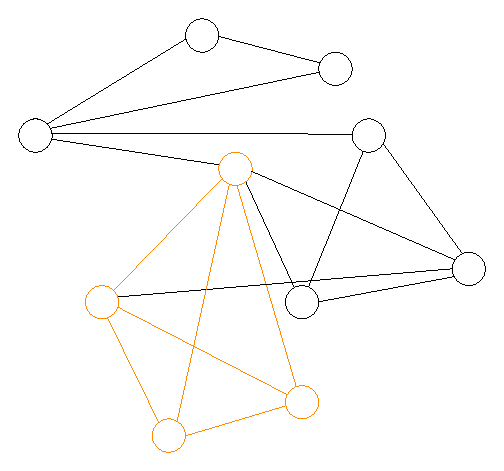
\includegraphics[width=0.3\textwidth]{graphics/graph1-clique.eps}
    \caption{A maximum clique.}
    \label{fig:maxclique}
\end{figure}

\begin{definition}[Maximum Clique Problem]
	\label{def:mcp}
	Given a graph $G = (V,E)$, the Maximum Clique Problem (MCP) is the problem of finding clique of maximum size in $G$. 
\end{definition}

\subsection{Relaxations of the MCP}

For some real-world applications, the MCP is too strict a model, as some applications require identifying large, dense subgraphs, but not necessarily fully connected subgraphs. 
Furthermore, it might be the case that acquiring real-world data is an error-prone process, thus requiring relaxations of the clique model tailored to the specific application. 
For these reasons, several relaxations of the maximum clique problem have been introduced: The Maximum $\gamma$-Quasi-Clique Problem \cite{Abello2002} and the Maximum $s$-Defective Clique Problem \cite{Yu2006} are density based and edge based relaxations, respectively, where a solution $S$ is a set of vertices with density of at least $\gamma$, or has at most $s$ edges missing in $G[S]$. 
The Maximum $s$-plex Problem is a degree based relaxation \cite{Seidman1978}, where each vertex in a solution $S$ is required to have at least $|S| - s$ neighbors in $S$, and the Maximum $s$-club Problem \cite{Mokken1979} is a path-based relaxation, where the induced subgraph $G[S]$ must have a diameter of at most $s$. Other relaxations include $s$-blocks, $s$-bundles and $s$-cores \cite{Gschwind2015}, among others. 

\subsection{Properties of the MCP}

In graph theory, a property $P$ of a graph $G$ is \textit{hereditary} if $P$ also holds for all induced subgraphs of $G$ \cite{pattillo_maximum_2013}. It is easy to see that the property of a graph being a clique is hereditary, as each subset of a clique is a clique itself. Heredity is an important concept in the context of graph theory, as it allows the development of algorithms that exploit the structure of solutions exhibited by heredity, e.g. \cite{Trukhanov2013} and \cite{GSCHWIND2018131}.  

Furthermore, there exist negative results about the hardness of approximating the maximum clique in a graph in polynomial time: In \cite{Hastad1999} and \cite{Zuckerman2007} the authors show that there exists no fully polynomial time approximation scheme for the MCP, unless $\mathit{P} = \mathit{NP}$, meaning that for a real number $\varepsilon > 0$ there exists no polynomial time algorithm that approximates the maximum clique in a graph with a factor of at least $O(n^{1-\varepsilon})$, where $n$ is the number of vertices in the input graph. More importantly, these hardness results are trivially also valid for relaxations of the MCP. Considering the hardness of approximability of the MCP and its relaxations, it is evident that heuristic approaches are of great importance when tackling large real-world instances that cannot be solved optimally in practice. 

\section{The Maximum Quasi-Clique Problem}\label{sec:mqcp}

The Maximum Quasi-Clique Problem (Definition \ref{def:mqcp}) is a density based relaxation of the MCP, which was first introduced by Abello et al. \cite{Abello2002}. Pattillo et al. show that for any $\gamma$ with $0 < \gamma < 1$, the problem is NP-complete in its decision variant \cite{pattillo_maximum_2013}. 

\begin{definition}[Maximum Quasi-Clique Problem]
	\label{def:mqcp}
	Given a graph $G = (V,E)$ and $\gamma \in (0,1]$, the Maximum $\gamma$-Quasi-Clique Problem (MQCP) is the problem of finding a subset of vertices $S \subseteq V$ of maximum size 
	such that the induced subgraph $G[S]$ has an edge density of at least $\gamma$, or, in other words, $G[S]$ contains at least $\gamma \binom{|S|}{2}$ edges. 
\end{definition}

\subsection{Properties of the MQCP}
In contrast to cliques, the property of being a quasi-clique is not hereditary. Algorithms which build upon heredity can therefore not easily be adapted to the MQCP. However, as noted in \cite{pattillo_maximum_2013}, quasi-cliques display a property which the authors call \textit{quasi-heredity}. A property $P$ of a graph $G = (V, E)$ is \textit{quasi-hereditary}, if there exists some $v \in V$ such that $G[V \setminus \{v\}]$ also has property $P$. Furthermore, the authors show that quasi-cliques are quasi-hereditary. Therefore, for a $\gamma$-quasi-clique of size $k$ there exists a series of $\gamma$-quasi cliques of size $1,2, \dots, k$ such that each $\gamma$-quasi clique is a strict subset of the next one. Most of the leading heuristic algorithms for the MQCP (e.g. \cite{djeddi_extension_2019}, \cite{zhou_opposition-based_2020}, \cite{chen_nuqclq_2021}) build upon this important property by searching for a sequence of $\gamma$-quasi cliques of increasing size in order to approximate the maximum $\gamma$-quasi clique in a graph. 

\subsection{Preprocessing of MQCP Instances}

In \cite{Abello2002}, the authors introduce the notion of $\gamma k$\emph{-peelable} vertices in the context of preprocessing. A vertex $v$ is $\gamma k$\emph{-peelable} if $v$ and all its neighbors have degree smaller than $\gamma k$. If a lower bound $k$ for the size of a maximum $\gamma$-quasi clique is known, the authors propose to remove all edges incident to $\gamma k$\emph{-peelable} vertices from $G$ in preprocessing. This preprocessing rule might be used to speed up the search process by sparsifying the graph, but we note that this preprocessing rule does not necessarily preserve the existence of optimal solutions. We prove this claim by giving a counterexample in Figure \ref{fig:preprocessing-mqcp-counterexample}, where the optimal solution cannot be obtained after applying said preprocessing rule. 


\begin{figure}
    \centering
    \begin{subfigure}{.5\textwidth}
      \centering
      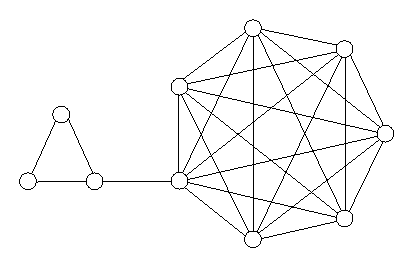
\includegraphics[width=.9\linewidth]{graphics/preprocessing-mqcp-counterexample-1.eps}
      \caption{The original graph instance.}
      \label{fig:preprocessing-mqcp-sub1}
    \end{subfigure}%
    \begin{subfigure}{.5\textwidth}
      \centering
      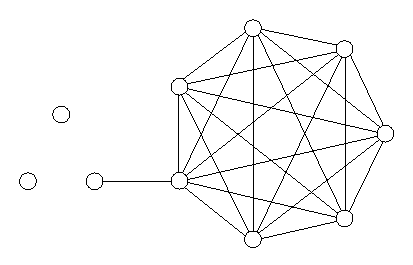
\includegraphics[width=.9\linewidth]{graphics/preprocessing-mqcp-counterexample-2.eps}
      \caption{The graph instance after preprocessing.}
      \label{fig:preprocessing-mqcp-sub2}
    \end{subfigure}
    \caption{Consider the graph $G$ given in Subfigure \ref{fig:preprocessing-mqcp-sub1}. The considered MQCP instance is defined by $G$ consisting of a $K_3$ and a $K_7$ connected by an edge and $\gamma=0.5$. Since $G$ has a density $dens(G) = \frac{25}{45} \approx 0.56$, the maximum $0.5$-quasi clique in $G$ is $V$. Assume a lower bound of $k=6$ is known, therefore the two vertices on the left are $k\gamma$\emph{-peelable} and preprocessing would remove all edges incident to these vertices, as can be seen in Subfigure \ref{fig:preprocessing-mqcp-sub2}. Therefore, the density of this preprocessed graph would be reduced to $\frac{22}{45} \approx 0.49$ and the optimal solution $V$ would not be preserved.}
    \label{fig:preprocessing-mqcp-counterexample}
\end{figure}

\section{The Maximum Defective Clique Problem}\label{sec:mdcp}

The Maximum Defective Clique Problem (\ref{def:mdcp}) was first introduced in \cite{Yu2006} in the context of predicting protein-protein interactions. 

\begin{definition}[Maximum $s$-defective-Clique Problem]
	\label{def:mdcp}
	Given a graph \\ 
    $G = (V,E)$ and integer $s$, the Maximum $s$-defective Clique Problem (MDCP) is the problem of finding a subset of vertices $S \subseteq V$ of maximum size 
	such that the induced subgraph $G[S]$ contains at least $\binom{|S|}{2} - s$ edges. 
\end{definition}

\subsection{Properties of the MDCP}

Although the MQCP and the MDCP are similar relaxations of the MCP, there are some key differences between the problems. It can easily be seen that the property of being a $s$-defective clique is hereditary: If $S$ is an $s$-defective clique with at most $s$ edges missing in $G[S]$, the removal of a vertex $v \in S$ cannot ``introduce'' any new missing edges.  
However, for a fixed size $k$, the two problems become interreducible: 
Finding a $k$-$s$-defective clique is equivalent to finding a $k$-$\gamma$-quasi clique with $\gamma = \frac{\binom{k}{2} - s}{\binom{k}{2}} $, and finding a $k$-$\gamma$-quasi clique is equivalent to finding a $k$-$s$-defective clique, where $s = \binom{k}{2} - \lceil \gamma \binom{k}{2} \rceil$. 
When approximating the maximum $s$-defective clique in a graph $G$ by a series of $s$-defective cliques of increasing size, the problem can therefore be reduced to finding a series of $\gamma$-quasi cliques and vice-versa.


% \section{The Maximum k-plex Problem}\label{sec:mpp}

% \todo{maximum k-plex problem}

% \begin{definition}[Maximum $k$-plex Problem]
% 	\label{def:mpp}
% 	Given a graph $G = (V,E)$ and integer $k$, the Maximum $k$-plex Problem (MPP) is the problem of finding a subset of vertices $S \subseteq V$ of maximum size 
% 	such that each $v \in S$ is adjacent to at least $|S| - k$ vertices in $S$. 
% \end{definition}


\chapter{Related Work}

Utilizing Machine Learning (ML) techniques in combinatorial optimization has been a research field of growing interest in recent years, and especially the application of graph neural networks (GNNs) in the context of combinatorial optimization is growing in popularity. 
In this chapter we want to provide a concise review of methods and work related to the topics of this thesis, namely ML methods and GNNs in combinatorial optimization, and also work related to the considered problems, the MCP, the MQCP, and the MDCP. Section \ref{sec:gnns} provides an introduction to the necessary concepts related to graph neural networks that are applied in this work, Section \ref{sec:ml-co} reviews the application of ML techniques that are relevant to this work, and \ref{sec:node-representation} presents methods to generate node features in feature-less graphs, which we apply in our algorithm in Chapter \ref{chp:gnn}. Furthermore, we provide an overview of existing heuristic and exact solution approaches for the MQCP in Section \ref{sec:mqcp-related-work} and for the MDCP in Section \ref{sec:mdcp-related-work}. 

\section{Graph Neural Networks}\label{sec:gnns}
% graph neural networks
Problems that are defined on graphs, e.g. the Traveling Salesperson Problem (TSP), pose new challenges in utilizing machine learning effectively: Utilized methods should be able to effectively capture and exploit the structure of input graphs, while taking into account that graphs do not have a unique representation and no fixed order of vertices, i.e. they should be \emph{order invariant}. Furthermore, graphs of all sizes should be considered as input, therefore utilized methods need to be \emph{scale invariant}. Ideally, the results of the training should generalize on unseen instances that might also be of different size than the instances seen during training. In order to address these challenges, researches have come up with machine learning architectures known as Graph Neural Networks (GNNs). 

The authors of \cite{Sperduti1997} were the first to research the application of neural networks on graphs. Since then, many researches have advanced the field by developing new architectures and methods. 
A comprehensive overview of the taxonomy of GNNs and a review of applications and methods can be found in \cite{Wu2019} and \cite{Zhou2020}. 

In \cite{Wu2019}, GNNs are classified into four main categories: Recurrent GNNs, Convolutional GNNs (ConvGNNs), Graph autoencoders, and Spatial-temporal graph neural networks. In the following, we conform to the authors' definitions of GNN-related concepts. 
In the context of our work, spatial-based ConvGNNs are the most relevant. 
The Message Passing Neural Network (MPNN) \cite{GilmerSRVD17} is a framework of spatial-based ConvGNNs, which captures several different concrete realizations due to its generality. 
Here, information corresponding to vertex $v$ in a graph is represented by a feature vector $x_v$, and convolution operations are defined to aggregate information of the neighboring vertices by passing messages over the edges of the graph. A convolutional layer then aggregates the features of neighboring vertices for all vertices in the graph. The general idea of this convolution operation is sketched in Figure \ref{fig:conv-gnn}, 
where the updated value for vertex $v_0$ is computed by aggregating the messages passed from its neighbors. MPNN uses a fixed number of layers to compute the final node embeddings. 
More precisely, to update the representation $h_v^{(k)}$ of a node $v$ in layer $k$, the following message passing function is applied: 

\[
    h_v^{(k)} = U_k (h_v^{(k-1)}, \sum_{u \in N_G(v)} M_k(h_v^{(k-1)}, h_u^{(k-1)}, x_{vu}^{e}))
\]
Here, $U_k(\cdot), M_k(\cdot)$ are functions with learnable parameters, $h_v^{(0)} = x_v$, and $x_{vu}^{e}$ is the feature vector of the (directed) edge from $v$ to $u$. Note that edge features are however not required, as also our work in this thesis utilizes spatial-based ConvGNNs on graphs that only contain information about vertices, but not about edges. 
The functions $U_k, M_k$ can be realized by any learnable function and thus cover many concrete realizations of the concept, for example $M_k$ can be an Multi-Layer Perceptron (MLP) that takes the concatenation of $(h_v^{(k-1)}, h_u^{(k-1)}, x_{vu}^{e})$ as inputs to compute its message, and $U_k$ is often realized by a ReLU activation function, followed by a batch-normalization \cite{IoffeS15} layer with learnable parameters. 

GNNs can be used for different tasks such as node-level tasks, e.g. the classification of nodes in a graph, edge-level tasks, e.g. edge classification or link prediction, or graph-level tasks, e.g. graph classification, both in supervised and unsupervised learning settings. 

\begin{figure}
    \centering
    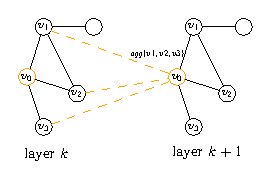
\includegraphics[width=0.5\textwidth]{graphics/gnn-conv.eps}
    \caption{Visual representation of the convolution operation for a vertex in a graph. Information of adjacent vertices is aggregated to compute the updated representation.}
    \label{fig:conv-gnn}
\end{figure}

\section{Machine Learning in Combinatorial Optimization}\label{sec:ml-co}

In many exact and heuristic algorithms for COPs, ML techniques are a determining factor in the effectiveness of said algorithms. There a many ways ML can be applied: It can be used in an end-to-end fashion to directly produce a solution, to replace or enhance key components of existing algorithms, to provide additional information to heuristics or metaheuristic, to obtain quick approximations for otherwise computationally heavy parts of an algorithm, or to make decisions within an algorithm, e.g. variable selection in branch-and-bound algorithms. A driving motivation in utilizing ML in COPs thus is to (partially) automate the process of hand-crafting heuristic algorithm components. 

Most of the current ML-based approaches are based on supervised learning, as stated in \cite{Cappart2021}. This often requires labeled training data in the form of optimal solutions to computationally hard problems, which is a great restriction. 
The two most common approaches to tackle this challenge are to either limit the training data to only incorporate labeled data of small instances that can be solved optimally within reasonable time, or to use high quality approximations, and thus decrease the solution quality. The former approach additionally poses the challenge to develop methods that translate well to unseen and possibly larger real-world instances that are relevant in practice. 
A prominent example of this application is \cite{Li2018}, where a GNN is trained to predict whether a vertex in the graph is in an optimal solution. A tree search algorithm is then executed that uses the information provided by the GNN. The approach generalizes well to instances that are much larger than those seen during training, and the authors apply it to multiple different COPs. 

Other approaches are based on unsupervised reinforcement learning and do not require labeled training data. 
In \cite{Khalil2017}, the authors propose an end-to-end reinforcement learning framework, S2V-DQN, which generalizes well to a wide range of problems. 
Furthermore, recent advances in this field have also been made by researchers of combinatorial games. Especially AlphaGo Zero is a prominent example, which was used to train models that excel in the board games Chess and Go via repeated self-play. AlphaGo Zero was later adapted in \cite{Abe2019} and applied to several combinatorial optimization problems, including Minimum Vertex Cover and Maximum Cut. 
In \cite{Kool2019} and \cite{Joshi2021}, the authors present end-to-end ML approaches by utilizing GNNs for routing problems including the Euclidean TSP. While their work shows promise, the proposed methods are only available for relatively small graphs, where exact approaches are available. In \cite{Hudson2021}, the authors present a guided local search approach, where a GNN is used to provide additional information to enhance the metaheuristic search, leading to improved results when applied to the TSP. Again, only relatively small instances are considered. 
We refer to \cite{Cappart2021} for a comprehensive overview of GNNs in the context of combinatorial optimization for both heuristic and exact algorithms. 

In the context of the MCP, several ML based approaches have been made. In \cite{Kristjan2022}, the authors build upon an exact branch-and-bound algorithm for the MCP, that uses an empirically determined algorithm parameter that greatly affects the algorithm's performance. The authors thus enhance the algorithm by training a GNN model to predict suitable parameter settings for each input graph. 
In \cite{Sun2021}, ML is applied to reduce MCP instances by training models to predict, whether a vertex is in an optimal solution or not. The input graph is then reduced, and an exact algorithm is applied to the reduced instance. 
Furthermore, in \cite{Yan2022}, the authors propose a metaheuristic breakout local search for the Maximum $k$-plex Problem (a degree-based MCP relaxation) that uses reinforcement learning in the diversification stage of the algorithm in order to predict good parameter settings for the diversification. Finally, a Pointer-Network based deep learning algorithm for the MCP is presented in \cite{Gu2020}. 
To the best of our knowledge, there are no ML-based or GNN-based approaches to the MQCP or the MDCP. 

\section{Node Representation Learning}\label{sec:node-representation}



\section{Solution Approaches for the MQCP}\label{sec:mqcp-related-work}

\subsection{Exact Approaches}\label{milp-mqcp}
Pattillo et al. \cite{pattillo_maximum_2013} propose a Mixed Integer Linear Programming formulation with a number of variables that is quadratic in the size of the vertex set $V$. 
It is derived from the following quadratic formulation, where $x_i \in \{0,1\}$ are binary decision variables representing the solution set $S \subseteq V$, and $a_{ij}$ represent elements of the adjacency matrix with $a_{ij}$ equal to one if $\{i,j\} \in E$ and zero otherwise: 

\fxnote{GR: MILPs schreibt man normalerweise so auf, dass die Zielfunktion und alle Funktionen linksbündig stehen, alle Quantoren rechtsbündig. Inequalities nicht in eine Zeile zusammenfassen (außer Domainangaben wie 0 <= x <= 10.)}
\begin{align}
    \max \sum_{i=1}^{n} x_i & \\
    \text{s.t. } \sum_{i=1}^n \sum_{j=i+1}^n a_{ij} x_i x_j & \geq \gamma \sum_{i=1}^n \sum_{j=i+1}^n x_i x_j
\end{align}
The authors linearize the above quadratic formulation by introducing variables $w_{ij}$ defined as $w_{ij} = x_i x_j$: 

\begin{align}
    \max & \sum_{i=1}^n x_i \\
    \text{s.t. } & \sum_{i=1}^n \sum_{j=i+1}^n (\gamma - a_{ij}) w_{ij} \leq 0  
\end{align}
\begin{align}
    w_{ij} &\leq x_i, & & w_{ij} \leq x_j, & & w_{ij} \geq x_i + x_j - 1, & & j > i=1, \dots , n \\
    w_{ij} &\geq 0,   & & x_i \in \{0,1\}, & & j > i = 1, \dots, n        & & 
\end{align}

\todo{try other MILP formulations: especially F3, F4 from \cite{VeremyevPBP16} seem interesting}

\subsection{Heuristic Approaches}

\subsubsection{Construction Heuristics}

\subsubsection{Population Based Heuristics}

\subsubsection{Local Search Based Metaheuristics}

\section{Solution Approaches for the MDCP}\label{sec:mdcp-related-work}


\chapter{A Local Search Based Metaheuristic for Maximum Clique Relaxations}\label{chp:local-search-algorithm}

In this chapter we present a local search based metaheuristic for relaxations of the MCP in detail, which is the algorithmic fundament of the GNN based algorithm in Chapter \ref{chp:gnn}
At first, we introduce the general structure of the algorithm without using GNNs in Section \ref{sec:algorithm-structure}. We present two types of construction heuristics that we use in our algorithm. The first one is used to efficiently obtain a feasible initial solution of high quality that can be used as a lower bound, whereas the second one does not necessarily yield a feasible solution, but is used to explore new regions of the search space not yet visited. In Section \ref{sec:neighborhood-structure} we define the main move operator used in the local search procedure and define the corresponding neighborhood structures. Furthermore, we show in detail the local search procedure of our algorithm that utilizes said neighborhood structures. 

\section{Algorithm Structure} \label{sec:algorithm-structure}

As noted by Friden et al. \cite{Friden1989}, a solution for the MCP can be obtained by finding a series of $k$-cliques for increasing values of $k$. Based on this observation, Wu et al. \cite{WuH13} develop an adaptive multistart tabu search algorithm for the MCP that in each iteration searches for a clique of size $k$ using a tabu search procedure. If such a clique can be found, $k$ is increased and the algorithm is restarted. The largest clique found this way is returned as the solution. Djeddi et al. \cite{djeddi_extension_2019} show that this idea can be extended to the MQCP by following the same principle: The maximum $\gamma$-quasi clique in a graph is approximated by finding a series of $k$-$\gamma$-quasi cliques, where the tabu search is restarted with increased $k$ each time a $k$-$\gamma$-quasi clique is found. This idea is applied successfully also in other state-of-the art algorithms for the MQCP, namely \cite{zhou_opposition-based_2020} and \cite{chen_nuqclq_2021}, which is why we want to base the general structure of our algorithm on this idea as well. 

The pseudocode of the general structure of our local search algorithm is shown in Algorithm \ref{alg:structure}.
$\mathit{InitialSolution}$, which is a generalized greedy search, constructs a feasible initial solution. Its main purpose is to obtain a high quality lower bound to obtain a good starting value for $k$. The procedure is described in detail in Section~\ref{sec:lower-bound-heuristic}.

In line \ref{alg:structure-freq} a long-term memory $\mathit{Freq}$ is initialized, where $\mathit{Freq[i]}$ stores how many times each vertex is operated on for $i=1,\dots,n$. This memory is kept when the loop in lines~\ref{alg:structure-while-start}--\ref{alg:structure-while-end} is repeated, but no feasible solution could be found. In $\mathit{ConstructionHeuristic}$, $\mathit{Freq}$ is used to produce a candidate solution that favors vertices that have not been considered yet. This way, new regions of the search space are explored. The idea of using this long-term memory $\mathit{Freq}$ in the construction heuristic to cover a larger area of the search space comes from \cite{chen_nuqclq_2021}. We change their construction heuristic slightly by combining it with a GRASP-like construction step as described in Section~\ref{sec:construction-heuristic}. 

Once a candidate solution is obtained by a construction heuristic, we try to improve it by the local search procedure in line~\ref{alg:structure-local-search}, which is described in detail in Section~\ref{sec:neighborhood-structure} along with the definition of the neighborhood structures. If the resulting solution $S$ is feasible, a simple search is performed in $\mathit{Extend}$ to check if the solution can be extended to a feasible solution of greater size as shown in Algorithm~\ref{alg:extend}.
Furthermore, $k$ is increased, $\mathit{Freq}$ is reset, and the best-so-far found solution $S^*$ is updated. 
If the solution obtained by the local search procedure is not feasible, the while-loop is repeated until the stopping criterion is met, e.g., the time limit is reached. 

\begin{algorithm}
    \DontPrintSemicolon
    \KwIn{Graph $G$, Target Density $\gamma$}
    \KwOut{Approximate maximum $\gamma$-quasi clique in $G$}
    $S^* \gets \mathit{InitialSolution}(G, \gamma)$ \;
    $k \gets |S^*|$ \; \label{alg:structure-lower-bound}
    $\mathit{Freq} \gets [0, \dots, 0]$ \label{alg:structure-freq} \tcp*{$n$-element Array, initialized with 0} 

    \While{stop condition not met}{ \label{alg:structure-while-start}
        $S \gets \mathit{ConstructionHeuristic}(G, \mathit{Freq}, k)$ \; \label{alg:structure-construction}
        $S \gets \mathit{LocalSearch}(G, Freq, \gamma, S)$ \; \label{alg:structure-local-search}
        \If{$S$ is feasible}{
            $S \gets \mathit{Extend}(G, S, \gamma)$ \;
            $S^* \gets S$ \;
            $k \gets |S| + 1$ \;
            $Freq \gets [0, \dots, 0]$ \; 
        }\label{alg:structure-while-end}
    }
    \Return{$S^*$}
    \caption{Structure of the Local Search Algorithm}
    \label{alg:structure}
\end{algorithm}

\begin{algorithm}
    \DontPrintSemicolon
    \KwIn{Graph $G$, Feasible solution $S$, Target Density $\gamma$}
    \KwOut{Feasible solution $S^\prime$ of size at least $|S|$}
    $S^\prime \gets S$ \;
    \While{$true$}{\label{alg:extend-while-start}
        \For{$u \in V \setminus S^\prime$}{
            \If{$S^\prime \cup \{u\}$ is a $\gamma$-Quasi Clique}{
                $S^\prime \gets S^\prime \cup \{u\}$ \;
                \textbf{continue} while-loop in line \ref{alg:extend-while-start} \;
            }
        }
        \textbf{break} out of while-loop
    }
    \Return{$S^\prime$}
    \caption{Extend a feasible solution}
    \label{alg:extend}
\end{algorithm}

\section{Lower Bound Heuristic}\label{sec:lower-bound-heuristic}

In this section we propose a beam search based heuristic that returns a feasible solution that can be used as a lower bound for the size of a maximum $\gamma$-quasi clique in the input graph. This lower bound is used to obtain a high starting value for $k$ in line~\ref{alg:structure-lower-bound} of Algorithm~\ref{alg:structure}. 
The pseudocode of the beam search is shown in Algorithm~\ref{alg:lower-bound-heuristic}. 
In the following, note the textual distinction between \emph{nodes} in the search tree and \emph{vertices} in the input graph which is made for the sake of clarity. 

In beam search, a node $v$ of the search tree is in general evaluated by a function $f(v) = g(v) + h(v)$, where $g(v)$ is the cost of the solution corresponding to a node, and $h(v)$ is a heuristically determined value given by a guidance function. 
We use a simple data structure for nodes of the search tree where a node $v$ has fields $\mathit{v.S}$ containing a feasible $\gamma$-quasi clique that this node represents, and $\mathit{v.h}$, which is the heuristically determined value of the node according to the used guidance function.
Additionally, we define the cost of a node $v$ as $g(v) = |v.S|$, which is the size of the feasible solution that this node represents.  
The root node of the beam search tree is then defined by an empty candidate set $\mathit{root.S}$ with $\mathit{root.g}=0, \mathit{root.h}=0$. 

The main loop in line~\ref{alg:exploration-construction-while-start}--\ref{alg:exploration-construction-while-end} expands all nodes in the current beam into feasible successor nodes. 
Since a node $v$ represents a set of vertices $\mathit{v.S}$ which is a feasible $\gamma$-quasi clique, successor nodes are generated by checking for each vertex $u \in V \setminus \mathit{v.S}$ whether $\mathit{v.S} \cup \{u\}$ is still a feasible $\gamma$-quasi clique. 
These successor nodes are then added to a list $\mathit{children}$. 
In order to keep the computational effort low, we introduce a parameter $\varepsilon$ that controls the maximum number of successor nodes for each node in the search tree. Thus, if a node has more than $\varepsilon$ feasible successors, we sort potential successors by the number of edges in their corresponding candidate solutions and add only $\varepsilon$ successor nodes to $\mathit{children}$, as can be seen in line \ref{alg:lower-bound-heuristic-expansion} of the algorithm.  

In order to avoid symmetries, i.e. nodes $u,v$ representing the same solutions such that $u.S = v.S$, we use a hash map for each level of the search tree containing all solution vertex sets that were already added for expansion. Before adding a successor node $v$ to $\mathit{children}$, a check is performed to make sure that a node representing $v.S$ is not already contained in $\mathit{children}$.  

Note that due to this expansion into successor nodes all the solutions corresponding to the nodes on a level of the search tree have the same cardinality, and thus the same $g$-value.  
Therefore, $g$-values can be ignored in the evaluation, and all nodes in $\mathit{children}$ are evaluated by a guidance function $h$, and the $\beta$ nodes with highest $h$-values form a new beam while the remaining nodes are discarded. 
Furthermore, since all the solutions corresponding to nodes on a level of the search tree have the same cardinality, a random node is selected to possibly update the best-so-far solution $S^*$ on each level.
Finally, when the beam becomes empty, the maximum cardinality solution is returned. 

We use the result of a simple greedy construction as the value of the heuristic function $h$: Given a node $v$ with candidate set $S = v.S$, greedily add the vertex $v = \arg \max_{u \in V \setminus S} d_S(u)$ if $S \cup \{v\}$ is still a feasible $\gamma$-quasi clique, where $d_S(u) = |\{v \mid v \in S, \{u,v\} \in E \}|$. 
Ties are broken randomly. This greedy extension is repeated until the corresponding solution is maximal, i.e., no single vertex can extend the cardinality of the solution while maintaining feasibility. 
The size of the solution obtained this way is then the return value of the guidance function $h(v)$. This greedy guidance function has a time complexity of $O(kn)$ per iteration, where $k$ is the solution size obtained by the greedy construction and $n$ is the number of nodes in $G$. 


    % \item The second guidance function takes a parameter $l$ and evaluates a node $v$ with candidate set $S = v.S$ by calculating the sum of the $l$ vertices in $V \setminus S$ with the highest values for $d_S(u)$. This guidance function is designed to be more time-efficient than the previous one, as the computation is independent of the solution size. 
    % \fxnote{braucht noch immer $O(n \log n)$ wegen sortieren und performt deutlich schlechter, vielleicht einfach rausstreichen?}


\begin{algorithm}
    \DontPrintSemicolon
    \KwIn{Graph $G$, Target density $\gamma$, guidance function $h$, beam width $\beta$, expansion control parameter $\varepsilon$}
    \KwOut{A feasible $\gamma$-quasi clique $S$}
    $\mathit{root.S} \gets \emptyset$ \;
    $S^* \gets \emptyset$ \;
    $\mathit{beam} \gets \{root\}$ \;
    \While{$\mathit{beam}$ not empty}{\label{alg:lower-bound-heuristic-while-start}
        $\mathit{children} \gets \emptyset$ \;
        \For{$\mathit{node} \in \mathit{beam}$}{
            Expand $\mathit{node.S}$ into up to $\varepsilon$ successor nodes that can be obtained by adding a vertex from $V \setminus \mathit{node.S}$ \; \label{alg:lower-bound-heuristic-expansion}
            $\mathit{children} \gets $ add feasible successor nodes obtained from expanding $\mathit{node}$ \;
        }
        \If{$children$ not empty}{
            $S^* \gets \mathit{node.S}$ for some arbitrary node in $\mathit{children}$ 
        }
        Evaluate nodes in $children$ by guidance function $h$ \;
        $\mathit{beam} \gets $ Choose $\beta$ nodes with highest $h$-values
    }\label{alg:lower-bound-heuristic-while-end}
    \Return{$S^*$}
    \caption{Lower Bound heuristic based on Beam Search}
    \label{alg:lower-bound-heuristic}
\end{algorithm}

\section{Construction Heuristic}\label{sec:construction-heuristic}

The construction heuristic in line \ref{alg:structure-construction} in Algorithm \ref{alg:structure} aims to return a set of nodes $S$ of fixed size $|S| = k$ that is promising to lead to new local optima when used as a starting point for the local search procedure. The candidate solution returned by this construction heuristic is not necessarily feasible. 
The construction heuristic includes a parameter $p \in [0,1]$ which controls the balance between choosing nodes that have not been explored yet and nodes that increase the objective value of the current candidate solution. This approach of balancing exploration and objective value is inspired by \cite{chen_nuqclq_2021}, where the authors use a similar strategy during construction. We combine the authors' idea with a GRASP-like approach. The procedure is shown in Algorithm \ref{alg:exploration-construction}. 
At first, a starting node is selected by choosing a node with the lowest $Freq$-value, breaking ties randomly. In each iteration of the main while loop in line \ref{alg:exploration-construction-while-start}-\ref{alg:exploration-construction-while-end}, with probability $p$ a node with the lowest $Freq$-value in $N_G(S)$ is added to the current candidate solution $S$. If $N_G(S)$ is empty, an arbitrary node with the lowest $Freq$ value from $V\setminus S$ is selected instead. 
With probability $1-p$ we perform an iteration of a GRASP-like randomized construction: A restricted candidate list $\mathit{RCL}$ is built by adding all nodes from $V \setminus S$ that fulfill the condition $d_S(u) \geq d_{\max} - \alpha(d_{\max} - d_{\min})$, where $d_S(u)$ denotes the number of neighbors in $S$ for a node $u \in V \setminus S$, and $d_{\max}, d_{\min}$ are the maximum and minimum values $d_S(u)$ over all nodes $u\in V \setminus S$. Here, the parameter $\alpha$ controls the balance between greediness and randomness in a GRASP-like manner: $\alpha=0$ corresponds to a greedy strategy, whereas $\alpha=1$ corresponds to a purely random strategy.  

\begin{algorithm}
    \DontPrintSemicolon
    \KwIn{Graph $G$, $n$-element array $Freq$, Target size $k$, GRASP parameter $\alpha$, Exploration parameter $p$}
    \KwOut{Candidate set $S$}
    $u \gets $ node in $G$ with lowest $Freq$-value, break ties randomly \;
    $S \gets \{u\}$ \;
    \While{$|S| < k$}{\label{alg:exploration-construction-while-start}
        \uIf{$rand() < p$}{
            \uIf{$N_G(S)$ not empty}{
                $u \gets$ Pick random neighbor in $N_G(S)$ with lowest $Freq$-value\;
            }
            \Else{
                $u \gets$ Pick random node in $V \setminus S$ with lowest $Freq$-value
            }
        }
        \Else{
            $d_{\min} = \min_{u \in V \setminus S} d_S(u)$ \;
            $d_{\max} = \max_{u \in V \setminus S} d_S(u)$ \;
            $RCL \gets \{ u \mid u \in V\setminus S, d_S(u) \geq d_{\max} - \alpha(d_{\max} - d_{\min}) \}$ \;
            $u \gets $ Pick random node from $RCL$ \;
        }
        $S \gets S \cup \{u\}$ \;
    }\label{alg:exploration-construction-while-end}
    \Return{$S$}
    \caption{Construction Heuristic with focus on exploration}
    \label{alg:exploration-construction}
\end{algorithm}

\section{Neighborhood Structure and Local Search} \label{sec:neighborhood-structure}

The neighborhood of a candidate solution $S$ is defined by a move operator that swaps a node $u \in S$ with a node $v \in V \setminus S$. The set of neighboring candidate solutions of $S$ with $|S| = k$ that can be obtained by a single swap move is therefore defined as $\Omega_1 = \{ S \setminus \{u\} \cup \{v\} \mid u \in S, v \in V \setminus S \}$ and has size $|\Omega_1| = k \cdot (|V|-k)$, which is in $O(|V|^2)$. Similarly, we define $\Omega_d$ for $d=1,2,3,\dots$ as the set of neighboring solutions that can be obtained by swapping $d$ nodes from $S$ with $d$ nodes from $V \setminus S$, obtaining a neighborhood of size $|\Omega_d| = \binom{k}{d} \cdot \binom{|V|-k}{d}$, which is in $O(|V|^{2d})$. 


The quality of a candidate solution depends on the considered problem. For the MQCP and the MDCP a candidate solution $S$ is of higher quality than a neighboring solution $S^\prime$ if $G[S]$ contains more edges than $G[S']$. Thus, we define the objective function $f \colon 2^V \rightarrow \mathbb{N}$ for the local search for MQCP and MDCP as the function that maps a subset of vertices $S \subseteq V$ to the number of edges in the induced subgraph $G[S]$. Therefore, $S$ is better than $S^\prime$ if and only if $f(S) > f(S^\prime)$. 

Similar algorithms that use local search in order to improve a candidate solution (e.g.,  \cite{chen_nuqclq_2021}, \cite{djeddi_extension_2019}, \cite{zhou_opposition-based_2020}) only search the neighborhood $\Omega_1$ for improving solutions. As the size of this neighborhood is already quadratic in $|V|$, the authors of the mentioned algorithms restrict the neighborhood to promising moves. A scoring function is used to find promising nodes in $V \setminus S$ and in $S$ that can be used for swaps. This scoring function is in most cases defined as $d_S(u) = |\{v \mid v \in S, \{u,v\} \in E \}|$. This way, the change in the objective function value when swapping a node $u \in S$ with a node $v \in V \setminus S$ can efficiently be calculated by $\Delta_{uv} = d_S(v) - d_S(u) - e_{uv}$, where $e_{uv} = 1$ if $\{u,v\} \in E$ and $e_{uv} = 0$ otherwise. 
The scoring function $d_S$ is thus used to restrict the neighborhood $\Omega_1$. 
Let $d_{\min} = \min_{u \in S} d_S(u)$ and $d_{\max} = \max_{u \in V \setminus S} d_S(u)$.
Furthermore, let 
\begin{align*}
    X &= \{ u \mid u \in S,~~~~~ d_S(u) \leq d_{\min} + 1 \}, \\
    Y &= \{ v \mid v \in V \setminus S, d_S(v) \geq d_{\max} - 1 \}.
\end{align*} The neighborhood $\Omega_1$ of a candidate solution $S$ is then restricted to only those neighboring solutions that can be obtained by swapping a node $u \in X$ with a node $v \in Y$, as all node swaps that maximize $\Delta_{uv}$ are contained in this restricted neighborhood. 

The pseudocode for our local search procedure is shown in Algorithm \ref{alg:local-search-procedure}. 
In each iteration of the main while-loop the restricted candidate sets $X$ and $Y$ are created from the sets $S$ and $V \setminus S$, respectively. These sets are created as described before, with an additional restriction: To prevent cycling through the same candidate solutions over and over again, a short-term memory is used to further restrict the sets $X$ and $Y$. There are two main methods that can be found in the literature, which we want to evaluate in our algorithm: 
\begin{itemize}
    \item In \cite{djeddi_extension_2019} and \cite{zhou_opposition-based_2020}, a tabu list is used to prevent cycling. Each time a vertex is added to or removed from the solution, it is added to the tabu list for a fixed number of iterations. While a vertex is in the tabu list, it is blocked and cannot be used in swaps. In \cite{djeddi_extension_2019}, the authors use two tabu lists: One for moving vertices out of the candidate solution, and one for adding vertices to the candidate solution. In \cite{zhou_opposition-based_2020}, a single tabu list is used for both operations. 
    \item In \cite{chen_nuqclq_2021}, the authors use Configuration Checking. In its simplest form, once a vertex $v$ is moved out of the candidate Solution, it is blocked from being moved again until at least one neighbor of $v$ is moved. The authors refine this strategy by using a threshold for each node $v$ that starts with $\mathit{threshold}(v) = 1$ for all $v \in V$. Each time a vertex $v$ is moved into the candidate solution, $\mathit{threshold}(v)$ is increased by 1. When $v$ is moved out of the candidate solution, it is blocked from being moved again, until $\mathit{threshold}(v)$ of its neighbors have been moved. Additionally, if $\mathit{threshold}(v) > \mathit{ub\_threshold}$, where $\mathit{ub\_threshold}$ is a user-defined upper bound, then $\mathit{threshold}(v)$ is reset to 1. 
\end{itemize}
If no improving move is possible, or one of the sets $X, Y$ is empty, a swap of two randomly selected unblocked vertices is performed in order to diversify the current local optimum. Furthermore, we define as stopping criteria: If the best solution $S^*$ does not improve for a fixed amount of iterations $\mathit{it}$, the procedure is stopped and $S^*$ is returned. Additionally, if a given time limit is reached, the procedure is stopped as well. 

\begin{algorithm}
    \DontPrintSemicolon
    \KwIn{Graph $G$, Frequency list $Freq$, Target density $\gamma$, Candidate solution $S$}
    \KwOut{Best found solution $S^*$}
    $k \gets |S|$ \;
    $S^* \gets S$ \;
    \While{stop criterion not met}{
        $X \gets $ restricted candidate set from $S$ \;
        $Y \gets $ restricted candidate set from $V \setminus S$ \;
        \uIf{$X$ or $Y$ empty}{
            Choose arbitrary unblocked $u \in S, v \in V \setminus S$\;
        }
        \uElseIf{there exists $u \in X, v \in Y$ with positive $\Delta{uv}$}{
            $u,v \gets $ Choose $u \in X, v \in Y$ with positive $\Delta{uv}$ \;
        }
        \Else{
            \tcp{No improving move possible}
            $u,v \gets $ Choose $u \in X, v \in Y$ arbitrarily
        }
        $S \gets $ solution obtained by swapping $u \in X, v \in Y$ \;
        Update $Freq[u], Freq[v]$ \;
        Update short-term memory \;

        \If{$f(S) > f(S^*)$}{
            $S^* \gets S$
        }
        \If{$S^*$ is feasible}{
            \Return{$S^*$}
        }
    }
    \Return{$S^*$}
    \caption{Local Search Procedure}
    \label{alg:local-search-procedure}
\end{algorithm}

Summarizing the previous sections, we present a flowchart visualization of the Local Search Based Metaheuristic presented in this chapter in Figure \ref{fig:flowchart-local-search-algorithm}. 

\begin{figure}
    \centering
    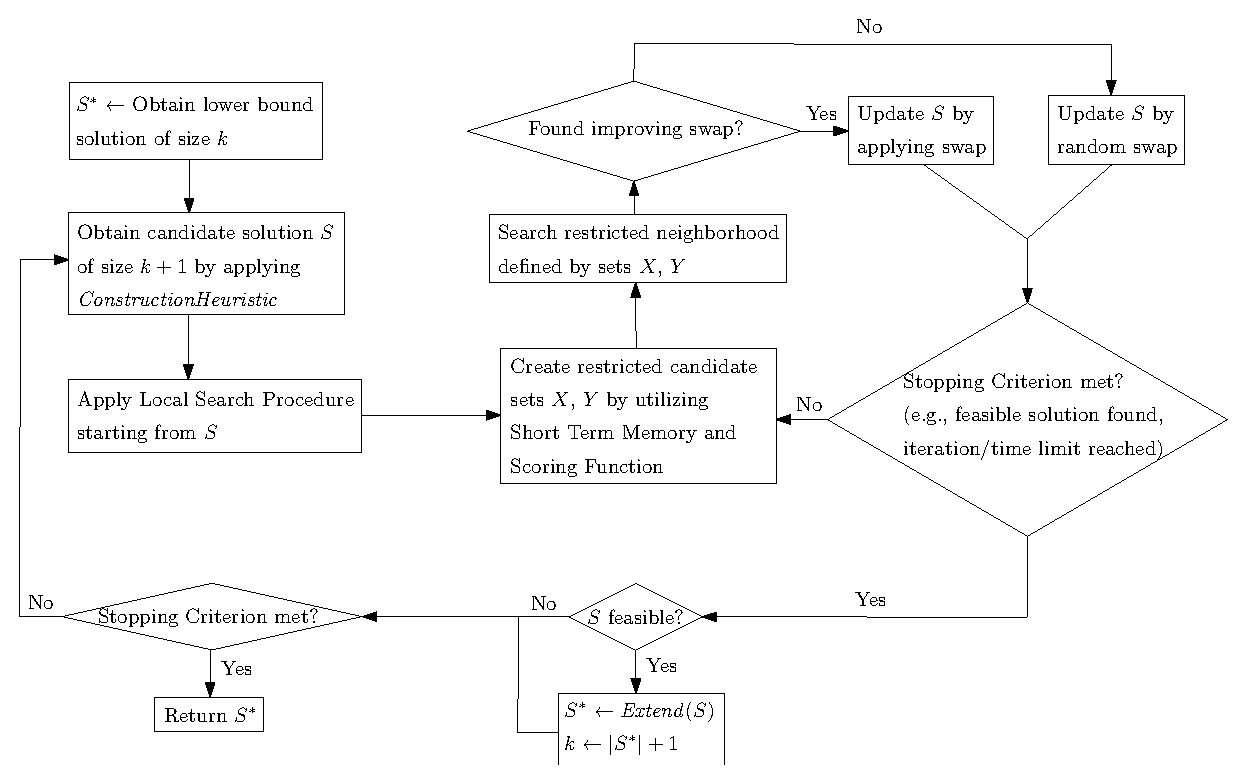
\includegraphics[width=\textwidth]{graphics/flowchart_local_search_algorithm.eps}
    \caption{Flowchart of the structure of the Local Search Based Metaheuristic.}
    \label{fig:flowchart-local-search-algorithm}
\end{figure}

\chapter{Using Graph Neural Networks in a Local Search Based Metaheuristic for Maximum Clique Relaxation Problems}\label{chp:gnn}

In this chapter we extend the local search based metaheuristic presented in Chapter \ref{chp:local-search-algorithm} by utilizing a GNN in order to enhance the algorithm. 
Section \ref{sec:gnn-local-search} presents our idea of utilizing a GNN in the previously described local search algorithm and the general structure of the training loop. 
Section \ref{sec:gnn-training} concerns the definition of training samples, and how training data is obtained. 
In order to obtain target values for training the GNN, in Section \ref{sec:lookahead-search} we present our idea of using a look-ahead search that takes into account the current candidate solution and returns the best neighboring solution. 
We discuss relevant GNN models and architectures in Section \ref{sec:gnn-architecture}. 
Finally, we analyze the effect of using a GNN as a scoring function on the runtime of the algorithm compared to the scoring function $d_S$ in Section \ref{sec:performance}. 


\section{Using a GNN in Local Search for Maximum Clique Relaxation Problems}\label{sec:gnn-local-search}

In Chapter \ref{chp:local-search-algorithm} we present a swap-based metaheuristic that evaluates possible swaps relative to a candidate solution $S$ by their respective gain $\Delta_{uv}$ for $u \in S, v \in V \setminus S$ which is similar to current state-of-the-art heuristic solution approaches. 
Here, the function $d_S$ can be seen as a scoring function over the vertices in $V$. Vertices with higher scores in $V \setminus S$ and vertices with low scores in $S$ are promising candidates for swapping, as they maximize the gain of a swap $\Delta_{uv}$. 
Most local search based algorithms on the MQCP are based around this scoring function, as it is efficiently computable, and swaps with a positive $\Delta_{uv}$ directly increase the objective value, which is the density of the candidate solution. 
Using $d_S$ as a scoring function to evaluate the quality of swaps has two major drawbacks:
\begin{itemize}
    \item In each iteration of the local search procedure, potential swaps are determined greedily: Only swaps that maximize the gain $\Delta_{uv}$ are considered. As discussed in Chapter \ref{chp:local-search-algorithm}, this corresponds to only searching the neighborhood structure $\Omega_1$. It is possible however, that one or more swaps with low gain lead to an improved solution - for example, a local optimum $S$ with respect to the neighborhood structure $\Omega_1$ is not necessarily a local optimum with respect to the neighborhood structure $\Omega_5$, and in order to obtain an improving solution from $S$ with respect to $\Omega_5$, some swaps might have a negative gain when applied consecutively. 
    \item As shown in \cite{chen_nuqclq_2021}, in most iterations there are many possible swaps with the same gain, but not all of them lead to the same local optima. In order to decide between swaps with equivalent gain the authors therefore propose to use a more fine-grained secondary scoring function which serves as a tiebreaker. 
\end{itemize}

In order to address these drawbacks, we propose to incorporate the GNN into the local search algorithm to enhance the function $d_S$ as a scoring function for swaps: In each iteration of the local search algorithm, all vertices are evaluated by a GNN, assigning scores to vertices. The GNN can therefore be seen as a function $\mathit{gnn}_S$, where $\mathit{gnn}_S(v)$ denotes the score of vertex $v$ relative to candidate solution $S$. 
As with $d_S$, the scores returned by the GNN induce a ranking over the possible swaps: High scores for vertices in $V \setminus S$ and low scores for vertices in $S$ indicate that these vertices are more likely to lead to an improved solution when considered for swaps. 
Moreover, note that $gnn_S$ is not necessarily independent of $d_S$: The $d_S$-values of vertices can be used as features for the vertices in the graph. Thus, function $d_S$ can also be taken into consideration, but its information is enhanced by structural information obtained from the graph in order to overcome its drawbacks. 

The purpose of the GNN in this approach is two-fold: 
\begin{itemize}
    \item Similar to the use of $d_S$, the scoring function $\mathit{gnn}_S$ can be used to restrict the neighborhood to only promising neighboring candidate solutions that can be obtained by only considering swaps involving the $k$ vertices with the highest scores in $V \setminus S$ with the $k$ vertices with the lowest scores in $S$. 
    \item The GNN can be trained to determine scores not only based on the neighborhood $\Omega_1$, but also to look ahead more than a single swap. This way, it can be used to obtain higher quality solutions as it is not caught in the local optima of the neighborhood structure $\Omega_1$.
\end{itemize}

Using a GNN however imposes some other challenges: 
Whereas the scoring function $d_S$ can be updated efficiently after a swap, incrementally updating the scores is generally not possible with a GNN, and obtaining scores therefore is less efficient using a GNN. 
Furthermore, the quality of the scores predicted by the GNN depends on several determining factors, most importantly on the quality of the training data and the obtained target values and the architecture of the GNN. 

We aim to tackle these challenges in Sections \ref{sec:gnn-training} and \ref{sec:lookahead-search} by showing how the GNN can be trained to make high quality predictions using principles from imitation learning and reinforcement learning, in \ref{sec:gnn-architecture} by proposing suitable efficient GNN architectures that can be used in practice, and in\ref{sec:performance} by analyzing the performance of the local search based metaheuristic with and without the GNN. 

\section{Training the GNN}\label{sec:gnn-training}

The general approach of the training algorithm is structured as depicted in Algorithm~\ref{alg:training}. A visualization of the algorithm structure is presented in the flowchart in Figure \ref{fig:flowchart-training-algorithm}. 
Starting with a naively initialized GNN, in each iteration of the training loop a random representative instance is generated on the fly and the local search algorithm is started with a fixed time limit. The local search algorithm is almost identical to the algorithm described in Chapter~\ref{chp:local-search-algorithm}, with the key difference that the GNN is used as a scoring function in order to restrict the neighborhood during search instead of the function $d_S$.  

During random iterations of the local search algorithm, training samples are added to a replay buffer, where a training sample consists of the graph $G$ and the current candidate solution $S$. For each training sample, a look-ahead search is applied in order to identify which vertices lead to improving solutions when considered for swaps. For a detailed description of how target values for these samples are computed, we refer to Subsection \ref{subsec:target-values} Section and \ref{sec:lookahead-search}, where we propose and discuss different methods to identify improving neighboring solutions. 
Once the time limit of the local search procedure is reached, the GNN is trained with data from the replay buffer. 
This process is repeated for $z$ iterations, until the GNN is sufficiently trained. 

Using the NN during training data generation is typical practice in reinforcement learning, where the NN is often improved by ``self-play''. 
We justify this algorithmic design choice by arguing about the trajectory of the search, i.e., the set of candidate solutions encountered during execution of the local search based metaheuristic with or without the GNN: using the GNN during training data generation will generate samples that would appear naturally during the execution of the local search based metaheuristic at test time. In contrast, using only $d_S$ as a scoring function during training data generation, the trajectory of the search might differ greatly compared to the trajectory when using the GNN - especially for an initially untrained GNN, which might decrease the stability of training. 

\begin{algorithm}
    \DontPrintSemicolon
    \KwIn{Untrained GNN $gnn$, Target density $\gamma$, Number of iterations $z$, min. replay buffer fill $\rho$}
    \KwOut{Trained GNN $gnn$}
    Initialize Replay Buffer $R$ \;
    \For{$z$ iterations}{
        $G \gets$ create representative graph instance \;
        $\mathit{LocalSearchWithTrainingDataGeneration}$($G$, $\gamma$, $gnn$, $R$) \;
        \If{$|R| > \rho$}{
            Train $gnn$ with data from $R$ \;
        }
    }
    \Return{$gnn$}
    \caption{Training the GNN}
    \label{alg:training}
\end{algorithm}

\begin{figure}
    \centering
    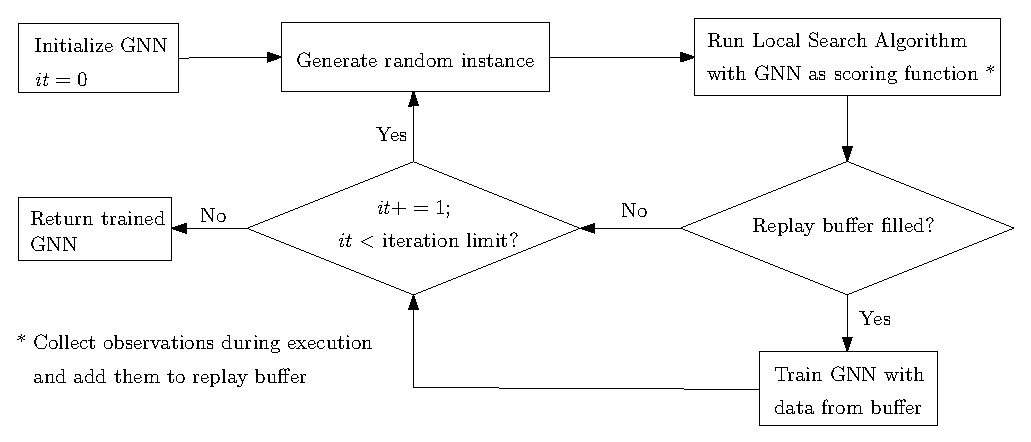
\includegraphics[width=\textwidth]{graphics/flowchart_training_algorithm.eps}
    \caption{Flowchart of the structure of the training algorithm.}
    \label{fig:flowchart-training-algorithm}
\end{figure}

\subsection{Obtaining Target Values}\label{subsec:target-values}
As already mentioned, a training sample consists of a graph $G = (V,E)$ and a candidate solution $S$. Training is done in an imitation learning setting: In order to obtain target values for the vertices in $V$, we apply a look-ahead search to the candidate solution $S$ as described in Section \ref{sec:lookahead-search}, and the GNN is then trained to imitate this look-ahead search. 
The look-ahead search returns a set of $j$ neighboring solutions $Y = \{S_1, S_2, \dots, S_j\}$ such that $S_1, S_2, \dots, S_j \subset V$ and $|S| = |S_1| = |S_2| = \dots = |S_j|$. Furthermore, all sets in $Y$ returned by the look-ahead search are the best neighboring solutions with respect to $S$ with equal objective value $f(S) < f(S_1) = f(S_2) = \dots = f(S_j)$. Note that if $S$ is already a local optimum with respect to the neighborhood structure searched by the look-ahead search, then $Y$ might be empty. Targets for the vertices in $V$ are then given by a mapping $y \colon V \rightarrow \{0,1\}$ which is defined the following way: For each $S_i \in Y$, let $S_{i}^1 = S_i \setminus S$, $S_{i}^0 = S \setminus S_i$. In other words, $S_i^1$ contains all vertices in $S_i$ that are outside $S$, and $S_i^0$ contains all vertices inside $S$ that are not in $S_i$. For $v \in (\bigcup_{S_i \in Y} S_i^1) \cup (S \setminus \bigcup_{S_i \in Y} S_i^0)$ we define $y(v) = 1$, and for $u \in \bigcup_{S_i \in Y} S_i^0$ we define $y(u) = 0 $. We demonstrate this mapping by a small example in Figure \ref{fig:target-values}. 

\fxnote{RE: Anmerkung von Günther: eventuell könnte man hier Prediction aufzuteilen in zwei Werte - 1. Knoten außerhalb von $S$, die hinzugefügt werden sollen, 2. Knoten innerhalb von $S$, die behalten werden sollen. Der derzeitige Ansatz funktioniert aber recht gut, daher wäre dieser Ansatz vielleicht später oder in zukünftiger Arbeit noch zu verfolgen. }

\begin{figure}
    \centering
    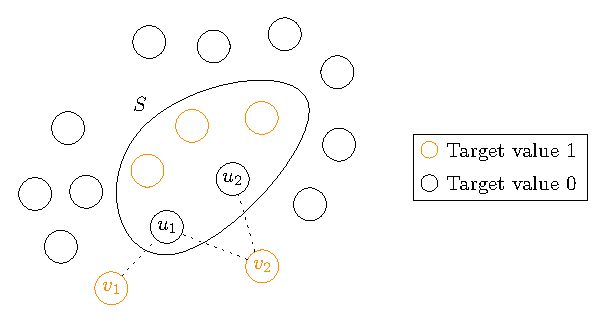
\includegraphics[width=0.8\textwidth]{graphics/target_values.eps}
    \caption[]{A training sample given by a graph $G$ with candidate solution $S$. Edges are omitted for the sake of clarity. The three best neighboring solutions of $S$ w.r.t. the $\Omega_1$ neighborhood structure can be obtained by applying one of the swaps $(u_1, v_1), (u_1, v_2), (u_2, v_2)$ (marked by dotted lines). Thus, the vertices $v_1, v_2$ and the vertices in $S \setminus \{u_1, u_2\}$ are labeled with 1, whereas all remaining vertices are labeled with 0. }
    \label{fig:target-values}
\end{figure}

As the target mapping $y$ maps the vertices to either 0 or 1, this method of training can be seen as a vertex level binary classification task. A vertex $v \in V \setminus S$ is labeled with 1, if there exists a vertex $u \in S$ with label 0 such that swapping $u, v$ leads to a candidate solution with improved objective value. 
In order to train the GNN we therefore propose to use the binary cross entropy\footnote{More precisely, we use Flux.jl's logitbinarycrossentropy function, which is mathematically equivalent, but more numerically stable} as a loss function, which is suitable for binary classification tasks:
\[
    \mathit{binarycrossentropy}(\hat{y}, y^\prime) = \mathit{mean}(-y^\prime \cdot \log(\hat{y} + \epsilon) - (1 - y^\prime) \cdot \log(1 - \hat{y} + \epsilon))    
\]
Here, $\hat{y}$ denotes a vector of size $|V|$ that contains predictions given by the GNN, $y^\prime$ denotes a vector containing the target values of vertices obtained as previously described using the mapping $y$, and $\epsilon$ denotes a small positive number that is included to avoid infinity. 

% Obtain target values: 
% \begin{itemize}
%     \item Imitation learning: 
%     \begin{itemize}
%         \item first appraoch: search neighborhood $\Omega_1$ for best solution(s). vertices in these solutions have target value 1, others have target value 0
%         \item extend first approach to a larger neighborhood, e.g. $\Omega_2$ or $\Omega_3$
%         \item for small graphs: use MILP model (implement better performing formulation F3 or F4 from \cite{VeremyevPBP16})
%         \item try beam search look ahead search, which also partially searches a larger neighborhood
%     \end{itemize}
%     \item Reinforcement learning:
%     \begin{itemize}
%         \item Beam Search with fixed depth $l$ to find best neighboring solution starting from candidate solution $S$: each node of the beam search tree corresponds to a candidate solution that has a distance of $i$ swaps to initial solution, where $i$ is the level of the search tree.
%         \item expand each node of the beam search tree into successor nodes that can be obtained by performing a single swap. expand each node into $k$ children, using the $k$ most promising swaps according to the GNN. this way the GNN guides how the search space is explored
%         \item evaluate each node by performing a single iteration of the local search procedure (with a local search / tabu search that uses the GNN as a scoring function). the value of a node is determined as the best found solution by the local search procedure
%         \item on each level, keep $\beta$ most promising nodes
%         \item when maximum depth $l$ is reached, return the candidate solution(s) that have the highest value according to the local search procedure. these solutions are then used as the best neighboring solutions 
%     \end{itemize}
%     \item If there is a single best neighboring solution, calculate training targets as described: 1 for vertices in best neighboring solution, 0 otherwise. As a refinement, use e.g. the 5 best neighboring solutions and calculate targets based on the objective value of each solution: e.g. 1 for nodes in the best solution, 0.8 for nodes in the second best solution, etc 
% \end{itemize}


\section{Look-Ahead Search}\label{sec:lookahead-search}

In order to obtain target values for training the GNN, we need to be able to identify the best neighboring solutions in a given neighborhood structure relative to the $S$. More specifically, we want to consider the neighborhood structure(s) $\bigcup_{i=1}^d \Omega_i$ for different values of $d$. In this section, we propose different methods in order to search these neighborhood structures. 

\subsection{A simple approach: Searching $\Omega_1$}

As a first approach, we can define the look-ahead search as simply searching the neighborhood structure $\Omega_1$ w.r.t. a candidate solution $S$, which can be done in time $O(|V|^2)$ by inspecting all possible swaps. Note that the optimization described in \ref{sec:neighborhood-structure} using the restriction of possible swaps to vertices from $X \subseteq S, Y \subseteq V \setminus S$ can be applied in order to speed up the search. 
When the GNN is trained successfully to imitate this look-ahead search, it will serve the same purpose as the function $d_S$ in Chapter~\ref{chp:local-search-algorithm}, as $d_S$ is used to efficiently search the neighborhood structure $\Omega_1$. 

\subsection{Beyond $\Omega_1$: Exact Approaches}

In order to search the larger neighborhoods $\bigcup_{i=1}^d \Omega_i$ for $d > 1$, we distinguish between exact approaches and heuristic approaches. 
In the remainder of this section, let $X_i \subseteq S, Y_i \subseteq V\setminus S$ be two sets of vertices of equal cardinality, and let $S^\prime = (S \setminus X_i) \cup Y_i$ be the neighboring solution of $S$ obtained by removing the vertices in $X_i$ from $S$ and adding the vertices in $Y_i$ to $S$. Let $\mathit{gain_S}(X_i, Y_i) = |E(G[S^\prime])| - |E(G[S])|$ denote the gain of edges when comparing $S^\prime$ and $S$.   

\subsubsection{Enumerating all possible swaps}
As already stated in Chapter \ref{chp:local-search-algorithm}, the neighborhood structure $\Omega_d$ contains $O(|V|^{2d})$ neighboring solutions and can be searched in time $O(|V|^{2d} \cdot T_d)$ by enumerating all possible swaps, where $T_d$ is the time needed for determining the objective value of a neighboring solution in $\Omega_d$. 
The $\mathit{gain_S}(X_i, Y_i)$ of a swap of nodes $X_i = \{u_1, \dots, u_d\}, Y_i = \{v_1, \dots, v_d\}$ is calculated using $d_S$ the following way: 
\begin{equation}\label{eqn:gain}
    \mathit{gain_S}(X_i, Y_i) = \sum_{u \in X_i} d_S(u) - \sum_{v \in Y_i} d_S(v) + |E(G[X_i])| + |E(G[Y_i])| - \sum_{u \in X_i} \sum_{v \in Y_i} e_{uv},
\end{equation}
where $e_{uv} = 1$ if $\{u,v\} \in E$, and $e_{uv} = 0$ otherwise. 
The above equation is a generalization of the calculation of $\Delta_{uv}$: When adding the vertices in $Y_i$ to the candidate solution $S$, we add $\sum_{u \in Y_i} d_S(u)$ edges between vertices in $Y_i$ and $S$, and $|E(G[Y_i])|$ edges between vertices in $Y_i$, from which we have to subtract $\sum_{u \in X_i} \sum_{v \in Y_i} e_{uv}$ edges between $X_i$ and $Y_i$, as the vertices from $X_i$ are removed from $S$. When removing the vertices in $X_i$ from $S$, we remove $\sum_{u \in X_i} d_S(u)$ edges, but the edges in $G[X_i]$ are counted twice, which is why we need to add the term $|E(G[Y_i])|$. Note that $T_d$ is in $O(d^2)$, as the number of summands in Equation \ref{eqn:gain} depends on $d$. 

We propose the following optimizations to speed up the search: 
\begin{itemize}
    \item Let $X_j = \{u_1, \dots, u_d\} \subseteq S, Y_j = \{v_1, \dots, v_d\} \subseteq V \setminus S$ such that $d_S(u_i) \leq u$ for $1 \leq i \leq d, u \in S \setminus X_j, d_S(v) \geq v$ for $1 \leq i \leq d, v \in V \setminus (S \cup Y_j)$, so $X_j$ contains the $d$ vertices in $S$ with the lowest $d_S$-values, and $Y_j$ contains the $d$ vertices in $V\setminus S$ with the highest $d_S$-values.  
    Then, for any sets of vertices $X_i = \{u_1, \dots, u_d\} \subseteq S, Y_i = \{v_1, \dots, v_d\} \subseteq V \setminus S$ it must hold that $\mathit{gain_S}(X_i, Y_i) \leq \sum_{v \in Y_j} d_S(v) - \sum_{u \in X_j} d_S(u) + 2 \cdot \binom{d}{2}$. If the upper bound on the right side of the inequality is less than or equal to zero, then $S$ is a local optimum with respect to $\Omega_d$, and it is not necessary to examine any of the neighboring solutions at all. 
    \item Similarly, we can derive a lower bound: Let $X_j, Y_j$ be as defined above. Then, $\mathit{gain_S}(X_j, Y_j)$ is clearly a lower bound for the maximum gain among all neighboring solutions of $S$. When calculating $\mathit{gain_S}(X_i, Y_i)$ for arbitrary sets $X_i = \{u_1, \dots, u_d\} \subseteq S, Y_i = \{v_1, \dots, v_d\} \subseteq V \setminus S$, we can therefore check, whether $\sum_{u \in Y_i} d_S(u) - \sum_{v \in X_i} d_S(v) + 2 \cdot \binom{d}{2} < \mathit{gain_S}(X_j, Y_j)$. If this is the case, we can avoid the computation of $\mathit{gain_S}(X_i, Y_i)$. This reduces the time $T_d$ from $O(d^2)$ to $O(d)$ if the above condition is fulfilled. 
\end{itemize}
% $d_S(v_{\sigma_{\max}(1)}) \geq \dots \geq d_S(v_{\sigma_{\max}(n)}), d_S(v_{\sigma_{\min}(1)}) \leq \dots \leq d_S(v_{\sigma_{\min}(n)})$

In practice, preliminary experiments have shown that searching the neighborhood exhaustively by enumeration of all possible swaps as described above is computationally infeasible for $d \geq 3$ even for small graphs ($|V| \leq 250$), even when applying the described optimizations. 

\subsubsection{MILP Approaches}

As an alternative approach, we present two MILP-formulations, which we adapted from the formulations presented in \cite{pattillo_maximum_2013} and in \cite{VeremyevPBP16}.
 
The first formulation is based on the first formulation in \cite{pattillo_maximum_2013}:  
\begin{align}
    \max & \sum_{i=1}^n \sum_{j=i+1}^n a_{ij} w_{ij} \\
    \text{s.t. } & \sum_{i \in V} x_i = k \label{milp:size-constraint} \\ 
     & \sum_{i \in S} x_i \geq k - d    \label{milp:branching-constraint}
\end{align}
\begin{align}
    w_{ij} &\leq x_i, & & w_{ij} \leq x_j, & & w_{ij} \geq x_i + x_j - 1, & & j > i=1, \dots , n \\
    w_{ij} &\geq 0,   & & x_i \in \{0,1\}, & & j > i = 1, \dots, n        & & 
\end{align}
We change the objective function to determine the neighboring solution $S'$ of $S$ that can be obtained after at most $d$ swaps and maximizes the amount of edges in $G[S']$. The equality in \ref{milp:size-constraint} ensures that the neighboring solution contains $|S| = k$ vertices, and the inequality in \ref{milp:branching-constraint} ensures that $|S' \setminus S| \leq d$. 

Furthermore, we also adapt the formulation F3 in \cite{VeremyevPBP16}, as the authors show both theoretically and empirically that the model performs better than the one in \cite{pattillo_maximum_2013}. This is done similarly as above, by introducing constraints \ref{milp:size-constraint} and \ref{milp:branching-constraint} and changing the objective function to maximize the number of edges in the solutions.  

In practice, we obtain similar results as for the exhaustive search of $\bigcup_{i=1}^d \Omega_i$: Even for relatively small graphs ($|V| \leq 250$), this method becomes infeasible for $d \geq 3$. 

\subsection{Beyond $\Omega_1$: Heuristic Approaches}

In order to make training feasible on larger instances and for greater $d$, we propose heuristic approaches that approximate the best neighboring solution, trading solution quality for efficiency. 

\subsubsection{Restricting the neighborhood}

Recall that during the execution of the Local Search Based Metaheuristic we restrict the cardinality of the sets of vertices $X \subseteq S, Y \subseteq V \setminus S$ to the $k$ vertices with the lowest and highest $\mathit{gnn}_S$-values, respectively. Similarly, when searching $\bigcup_{i=1}^d \Omega_i$, we can restrict the cardinality of the sets of vertices considered for swaps $X, Y$ to contain up to $k^\prime$ vertices with the lowest and highest $\mathit{gnn}_S$-values each, and then exhaustively enumerate all possible neighboring solutions that can be obtained by removing up to $d$ vertices in $X$ from $S$ and adding up to $d$ vertices from $Y$. Intuitively, it makes sense to use a value $k^\prime > k$, as this means a greater part of the neighborhood structure $\bigcup_{i=1}^d \Omega_i$ is explored and therefore the approximation is more likely to be precise. 
Furthermore, by using a fixed size neighborhood determined by $k^\prime$, the computation scales well on larger graphs. 
In order to make this training process more stable, we propose to start training with targets computed by searching a small neighborhood like $\Omega_1$ that can be searched exhaustively without restriction, and then changing to a restricted, bigger neighborhood.  

\subsubsection{A Beam Search Based Approach}

 This method is based on Beam Search and its pseudocode is shown in Algorithm \ref{alg:lookahead-beam-search}.
 We define a simple data structure for nodes in the beam search tree, where each node $v$ in the search tree corresponds to a set $S^\prime$ that can be obtained from the candidate solution $S$ by removing the vertices in $v.in \subseteq S$ from $S$ and adding the vertices in $v.out \subseteq V\setminus S$ to $S$. 
 Typically, each node $v$ in the beam search tree is evaluated by an evaluation function $f(v) = g(v) + h(v)$, where $g(v)$ denotes the cost of $v$ and $h(v)$ denotes a heuristic value determined by the heuristic guidance function $h$. In Algorithm \ref{alg:lookahead-beam-search}, we define $g(v)$ to be the number of edges in the solution $S^\prime$ that corresponds to $v$, and we set $h(v) = 0$ for all nodes in the search tree. 

In each iteration all nodes representing candidate solutions in the beam are expanded into child nodes the following way: Assume a candidate solution $S^\prime$ corresponds to a node $v$ in the search tree. This node $v$ is then expanded into up to $\varepsilon^2$ successor nodes that can be obtained by adding on of the $\varepsilon$ vertices with highest $d_{S^\prime}$-values in $(V \setminus S^\prime) \setminus v.\mathit{in}$ to $v.out$ and one of the $\varepsilon$ vertices with the lowest $d_{S^\prime}$ values in $S^\prime \setminus v.\mathit{out}$ to $v.in$. Note that the vertices in $v.in, v.out$ are excluded in order to avoid repeating candidate solutions. All expanded nodes are then evaluated by their $f$-values and the $\beta$ nodes with highest $f$-values become the new beam, whereas the remaining solutions are discarded. 

Note that by the described expansion of the nodes into successor nodes, each level $i$ of the search tree only contains nodes that can be reached by performing exactly $i$ swaps from the root node which corresponds to the initial candidate solution $S$. 
In order to avoid symmetries, i.e. performing the swaps $(u_1, v_1), (u_2, v_2)$ produces the same candidate solution as performing the swaps $(u_1, v_2), (u_2, v_1)$, we use a hash map for each level of the search tree that stores the sets $v.\mathit{in}, v.\mathit{out}$ for each node. This way, when expanding a node $v$ into its successor nodes, we can check efficiently, whether a node with matching sets $v.\mathit{in}, v.\mathit{out}$ have already been added to $\mathit{children}$.  

This process is continued, until a fixed depth $d$ is reached in the search tree. The candidate solution with the highest $f$-value is then returned. Note that this approach can easily be adapted to return multiple solutions if there are multiple best solutions with the same $f$-value. 


\begin{algorithm}
    \DontPrintSemicolon
    \KwIn{Graph $G$, candidate solution $S$, Depth $d$, Expansion factor $\varepsilon$, beam width $\beta$}
    \KwOut{Neighboring candidate solution $S^*$ that approximately maximizes the objective function}
    $\mathit{root}.f, \mathit{root}.\mathit{in}, \mathit{root}.\mathit{out} \gets f(\mathit{root}), \emptyset, \emptyset$ \;
    $\mathit{max\_node} \gets \mathit{root}$ \;
    $\mathit{beam} \gets \{\mathit{root}\}$ \;
    \While{$\mathit{beam}$ not empty and $d > 0$}{
        $d \gets d-1$ \;
        $\mathit{children} \gets \emptyset$\;
        \For{$\mathit{node} \in \mathit{beam}$}{
            $S^\prime \gets $ solution corresponding to $\mathit{node}$ \;
            $X \gets $ select $\varepsilon$ vertices in $S^\prime \setminus \mathit{node}.\mathit{out}$ with lowest $d_{S^\prime}$-values \;
            $Y \gets $ select $\varepsilon$ vertices in $V \setminus (S^\prime \cup \mathit{node}.\mathit{in})$ with highest $d_{S^\prime}$-values \;
            \For{$(u,v) \in X \times Y$}{
                $\mathit{child\_node} \gets f(child_node), \mathit{node}.\mathit{in} \cup \{u\}, \mathit{node}.\mathit{out} \cup \{v\}$
                Add $\mathit{child\_node}$ to children if no node with $\mathit{child\_node}.\mathit{in}, \mathit{child\_node}.\mathit{out}$ exists in $\mathit{children}$
            }
        }
        $\mathit{beam} \gets $ select $\beta$ nodes with highest $f$-value \;
        \If{$\mathit{beam}$ not empty}{
            $\mathit{max\_beam} \gets \arg\max_{\mathit{node} \in \mathit{beam}} \mathit{node}.f$ \;
            \If{$\mathit{max\_beam}.f > \mathit{max\_node}.f$}{
                $\mathit{max\_node} \gets \mathit{max\_beam}$ \;
            }
        }
    }
    $S^* \gets$ obtain solution from $S, \mathit{max\_node}$ \;
    \Return{$S^*$}
    \caption{Beam Search based look-ahead search}
    \label{alg:lookahead-beam-search}
\end{algorithm}

\section{GNN Architecture}\label{sec:gnn-architecture}
In this section we present the key components of the GNN architecture used in our algorithm and justify our choices in designing said architecture. 
The whole process of evaluating a graph $G = (V, E)$ and a candidate solution $S$ is presented by means of a small example in Figure \ref{fig:gnn-architecture}. 
Initially, feature vectors $x_1, \dots, x_n$ are computed for all vertices in $V = \{v_1, \dots, v_n\}$, producing a feature matrix of dimension $\mathit{dim_{in}} \times |V|$, where $\mathit{dim_{in}}$ is the size of a feature vector. This feature matrix is used as input for the GNN based encoder, which consists of $l_e$ graph convolutional layers and outputs a node embedding matrix of dimension $\mathit{dim_{out}} \times |V|$. From these node embeddings, a context is computed by taking into account the current candidate solution $S$, and aggregating corresponding node embeddings by an aggregation function $\mathit{agg}$, generating a context embedding. The context embedding and the $d_S$-values for the vertices in $V$ are then concatenated to the node embeddings. The resulting matrix is used as input for the decoder, which can be realized as an MLP with a final layer $l_d$, which maps the values of the previous layer to a scalar output score by applying a sigmoid activation function. 

In the remaining Section we will discuss feature selection, the structure of the encoder and decoder, and the context embedding in detail. 

\begin{sidewaysfigure}
    \centering
    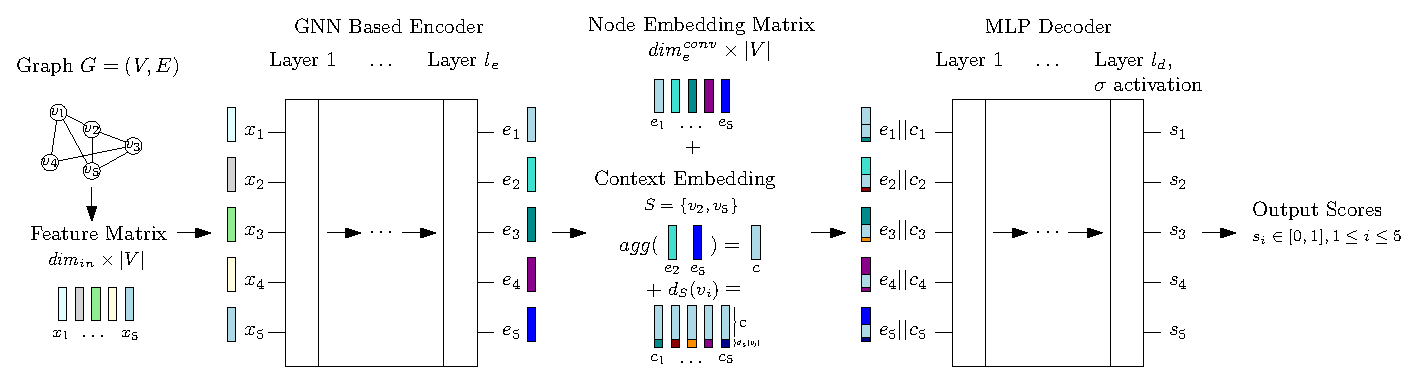
\includegraphics[width=0.9\textwidth]{graphics/gnn-architecture.eps}
    \caption{Evaluation of a graph $G = (V, E)$ with candidate solution $S = {v_2, v_5}$ by the Encoder-Decoder based architecture. }
    \label{fig:gnn-architecture}
\end{sidewaysfigure}

\subsection{Node Features}
Since the node embeddings are only computed once per graph, it is essential that the computed node features represent the vertices in a meaningful way by extracting similarities and differences of vertices and their surrounding neighborhoods. More precisely, high quality features should map vertices with similar neighborhoods closer together in the feature space, whereas vertices that are very distant from each other and do not share any structural similarities should be further apart. Moreover, it is essential that the chosen feature initialization method is generalizes well on unseen graphs, as the GNN used in our algorithm is trained offline on representative problem instances that differ from the instances encountered during execution. 

In \cite{Duong2019} the authors analyze the effect of different node feature initialization methods on node classification task. They distinguish between centrality based approaches (e.g. degree based initialization, number of triangles that a vertex participates in, etc), and learning-based approaches (e.g. DeepWalk \cite{Perozzi2014}, where vertices are mapped closer together, if the probability that they occur in a random walk together is higher). 
The authors conclude that centrality-based approaches are generally not as suitable as learning-based approaches by evaluating different feature initialization approaches in a node classification setting. 
We therefore investigate both the application of centrality-based and learning-based feature initialization methods. 

For centrality-based features, we evaluate \emph{Degree} initialization, where each vertex is initialized by its degree, and \emph{EgoNet} initialization: Given a graph $G = (V, E)$, and vertex $v \in V$, let $N(v, d)$ be the set of vertices reachable from $v$ by a path of length at most $d$. The induced subgraph $G[N(v, d)]$ is the $d$-hop-EgoNet of vertex $v$. Note that for $d=1$, $N(v, d)$ is the closed neighborhood of $v$ in $G$. We derive three features from the EgoNet of each vertex in $V$: the size $|N(v, d)|$, the number of edges in the subgraph induced by the EgoNet $|E(G[N(v, d)])|$, and the number of edges that leave $N(v, d)$, i.e. ${\{u, v\} \mid u \in N(v,d), v \notin N(v,d), \{u,v\} \in E}$.     

Learning-based feature initialization models are mostly based on generating variations of random walks on the original graph or a derived graph, and then mapping vertices closer together in the feature space that often occur in these random walks together at a certain distance. Notable methods are \emph{DeepWalk} \cite{Perozzi2014}, its generalization \emph{Node2Vec} \cite{GroverL16} that introduces hyperparameters for the random walks, and \emph{Struct2Vec} \cite{FigueiredoRS17}. Whereas DeepWalk and Node2Vec take locality and distance between vertices into account, Struct2Vec is focused on structural similarities, i.e. vertices with structurally similar neighborhoods are mapped closer together, even though they can be at a great distance in the actual graph. We therefore propose to evaluate different parameterizations of Node2Vec and Struct2Vec in the context of our algorithm. 

\subsection{Encoder}
In general, any graph convolutional network (GCN) model can be used as an encoder. We refer to Residual Gated Graph Convolutional Networks (\cite{Bresson2017}), and GATv2 networks (\cite{Velickovic2018}, \cite{Brody2021}), which we will use in our experiments. Based on these GCN models, we propose two architectures. In the following we denote by $dim_i$ the input dimension of layer $i, 0 \leq i \leq l_e$ of the network, where $l_e$ is the number of layers used in the encoder, $dim_0$ corresponds to the feature dimension of the node features, and for $1 \leq i \leq l_e$ $dim_i$ corresponds to the output dimension of layer $i$. 

\subsubsection{Residual Gated Graph Convolutional Encoder}
The update function of a Gated Graph Convolutional layer is defined in \cite{Bresson2017} as 
\[
    h_i^{l+1} = f_{\text{G-GCNN}}^l(h_i^l, \{ h_j^l \colon j \rightarrow i \}) = \text{ReLU} \Big( U^l h_i^l + \sum_{j \rightarrow i} \eta_{ij} \odot V^l h^l_j \Big),
\]
where $\eta_{ij} = \sigma(A^l h_i^l + B^l h_j^l)$. Here, $A^l, B^l, U^l, V^l$ are learnable parameter matrices and $\odot$ denotes the hadamard-product. 
Furthermore, the authors define the Residual Gated Graph Convolutional layer by adding the identity operator: 
\[
    h_i^{l+1} = f_{\text{G-GCNN}}^l(h_i^l, \{ h_j^l \colon j \rightarrow i \}) + h_i^l
\]
The authors suggest that residual layers should be used on successive convolutional layers. 
We add a batch normalization (\cite{IoffeS15}) layer after every GCN layer, which results in a final update function 

\[
    h_i^{l+1} = \text{BN} \Big( f_{\text{G-GCNN}}^l(h_i^l, \{ h_j^l \colon j \rightarrow i \}) + h_i^l \Big),
\]
where BN denotes batch normalization. 

We therefore propose a GCN model \textit{RG-GCN}, which makes use of these layers and is structured as follows: 
\begin{itemize}
    \item Layer 0: We apply a learnable linear transformation with weight matrix $A_0$ and bias vector $b_0$, these weights are shared among all vertices. 
    \item Layer 1: We apply a Gated Graph Convolutional layer that maps the feature vectors of dimension $dim_0$ to embeddings of dimension $dim_1$, followed by batch normalization.
    \item Layers 2, \dots, $l_e$: For layer $i, 2 \leq i \leq l_e$ we apply a Residual Gated Graph Convolutional layer, followed by batch normalization, mapping inputs of dimension $dim_{i-1}$ to dimension $dim_i$. 
\end{itemize}

\subsubsection{GATv2 Encoder}
We build upon the work of \cite{Kool2019}, in which the authors also use the Graph Attention Network architecture:
\begin{itemize}
    \item Layer 1: We apply a linear transformation $A_1 x_i + b_1$ with learnable parameters $A_1, b_1$ for each feature vector $x_i, 1 \leq i \leq n$.
    \item Layers 2, \dots, $l_e$: Following the GCN model used by \cite{Kool2019}, each attention layer consists of two sub-layers: A multi-head attention (MHA) layer and a dense, fully connected feed-forward (FF) layer. Each sub-layer also applies a skip-connection and batch-normalization. The following sub-layer definitions are given by the authors: 
    \begin{align*}
        \hat{h}_i &= \text{BN}^l(h_i^{(l-1)} + \text{MHA}_i^l (h_1^{(l-1)}, \dots , h_n^{(l-1)}) ) \\
        h_i^{(l)} &= \text{BN}^l(\hat{h}_i + FF^l(\hat{h}_i))
    \end{align*}
\end{itemize}
The authors in \cite{Kool2019} use as the MHA layer an attention mechanism which is based on the transformer architecture in \cite{VaswaniSPUJGKP17}, which we replace by the newer GATv2 layer from \cite{Brody2021}

\subsection{Context}
The context is determined by the current candidate solution $S$ and is computed by aggregating the columns of the node embedding matrix that correspond to the vertices in $S$. In general, any order invariant aggregation function $\mathit{agg} \in \{\mathit{sum, mean, max}\}$ can be used. Furthermore, we derive features from the function $d_S$ (the $d_S$-values can of course be used, but also the mean and standard deviation of all $d_S$-values might be valuable information) and append them to the context embeddings, creating feature vectors $e_i ||c_i$ for $v_i, 1 \leq i \leq |V|$ by concatenating the context and the node embeddings. These final embeddings are used as inputs for the decoder. 

\subsection{Decoder}
The decoder is a regression model that maps the inputs obtained from the node embeddings and the context embedding to scalar values representing scores for the vertices in $V$. We suggest using a simple MLP architecture with a sigmoid activation function on the final layer, mapping the results of the previous layers to scalar values between zero and one. 

As an addition to the node embeddings and the context embedding, the current $d_S$-values can also be used as decoder inputs. Furthermore, as the decoder evaluates each vertex independently, it might also be relevant to add information about the distribution of the $d_S$ values, e.g. mean and standard deviation. 

\section{Performance}\label{sec:performance}

Since the main difference between the algorithms presented in Chapter \ref{chp:local-search-algorithm} and \ref{chp:gnn} lies in the scoring function used to evaluate vertices during the swap based local search procedure, we want to analyze the effect of using the scoring function $\mathit{gnn}_S$ instead of the scoring function $d_S$. 
In order to do so, we identify the three main operations during the local search procedure that are influenced by the choice of scoring function: Initialization, restricting neighborhoods, and updating the scoring function.  

\subsection{Initializing the scoring function}
At the start of the local search procedure, a construction heuristic is used to produce a new candidate solution $S$, which serves as a starting point. 
The scoring function $d_S$ must then be initialized, as it is dependent on $S$. The initialization procedure can be seen in Algorithm \ref{alg:init-dS}.
It starts by initializing an array of zeros of size $|V|$. For each vertex $u \in S$, increase the value $d_S[v]$ by one for each neighbor $v$ of $u$. This procedure has a worst-time-complexity of $O(|V|^2)$ time, as the size of $S$ is in $O(|V|)$, and each vertex in $S$ can have $O(|V|)$ neighbors. 

\begin{algorithm}
    \DontPrintSemicolon
    \KwIn{Graph $G = (V,E)$, candidate solution $S$}
    \KwOut{Initialized scoring function $d_S$}
    $d_S \gets [0, \dots, 0]$ // Array of size $|V|$ \;
    \For{$u \in S$}{
        \For{$v \in N_G(u)$}{
            $d_S[v] \gets d_S[v] + 1$
        }
    }
    \Return{$d_S$}
    \caption{Initialize scoring function $d_S$}
    \label{alg:init-dS}
\end{algorithm}

When using the scoring function $gnn_S$, initializing the scoring function is done by computing node embeddings for each vertex in $G$. This is done by first computing node features and then computing node embeddings by passing the node features through a GNN based encoder. The time complexity of this initialization depends on the complexity of the chose node features and the structure of the GNN itself, but in general both will take $O(|V|^2)$ time on graphs that are not sparse. The argument is similar as with $d_S$, as each vertex needs to be evaluated by taking into account all its neighboring vertices. 
The advantage when using a GNN based scoring function is that this initialization process has to be done only once per graph, and not every time a new candidate solution is generated by the construction heuristic. In subsequent restarts of the local search procedure, only the linear time decoder has to be applied. 

Since initialization is only done once per graph or once per restart of the local search procedure, the runtime should not have a great impact on the performance of the algorithm. Therefore, especially with a GNN based scoring function, this time should be used by utilizing an encoder of high enough complexity to produce high quality node embeddings. 

\subsection{Restricting the neighborhood}
When using the scoring function $d_S$, the neighborhood $\Omega_1$ is searched implicitly, as only swaps that maximize the gain are considered. 
The restricted candidate sets $X \subseteq S, Y \subseteq V \setminus S$ are generated in time $O(|V|)$, as only the minimum and maximum scores for vertices in $S$ and $V \setminus S$, respectively, have to be determined. As a reminder, the restricted candidate sets are defined as 
\[
    X = \{ u \mid u \in S, d_S(u) \leq d_{\min} + 1 \}, \\
    Y = \{ v \mid v \in V \setminus S, d_S(v) \geq d_{\max} - 1 \},
\]
with $d_{\min} = \min_{u \in S} d_S(u), d_{\max} = \max_{v \in V \setminus S}$. 
If the swap $u \in S,v \in V \setminus S$ maximizes the gain of the candidate solution, this method of restricting the neighborhood guarantees that $u \in X, v \in Y$.
While this method produces restricted neighborhoods of variable size, these neighborhoods are usually small and thus can be searched efficiently in practice. In general however, the size of the sets $X, Y$ can be in $O(|V|)$ in the worst case. 

Using the scoring function $\mathit{gnn}_S$, we do not have a guarantee that the swap that maximizes the gain lies among the lowest-scoring vertices in $S$ and the highest-scoring vertices in $V \setminus S$. Moreover, we might not even want to consider such a swap, as the scoring function was trained to search greater neighborhoods than $\Omega_1$, and the swap that maximizes the gain does not lead to the best neighboring solution. We therefore propose to use restricted candidate sets $X,Y$ of a fixed size $k$, where $X$ consists of the $k$ lowest-scoring vertices in $S$, and $Y$ consists of the $k$ highest-scoring vertices in $V \setminus S$. This guarantees that searching the neighborhood takes a fixed amount of time. 
Obtaining the $k$ highest or lowest scoring vertices can be done in time $O(k |V|)$, which is linear for fixed $k$, but is still more expensive than generating a restricted neighborhood for the scoring function $d_S$. As the restricted neighborhood is searched in every iteration of the local search procedure, its size can therefore also have a great impact on the runtime. It is therefore essential to determine a neighborhood size that strikes a good balance between efficiency and quality of neighboring solutions found in the neighborhood.  


\subsection{Updating the scoring function}
After each swap of vertices $u \in S, v \in V \setminus S$ the scoring function needs to be updated, as it is dependent on the current candidate solution $S$. For $d_S$, this update can be efficiently in $O(|V|)$ time by decrementing $d_S[x]$ for $x \in N_G(u)$ and incrementing $d_S[y]$ for $y \in N_G(v)$. All other vertices remain unaffected by a single swap and their corresponding $d_S$-values do not need to be updated. 

For the scoring function $gnn_S$, we can generally not update the scores incrementally, as the context embedding changes, which is part of the input of all vertices. Therefore, all vertices need to be re-evaluated by the decoder. This still takes time linear in the number of vertices, but, depending on the complexity of the decoder, it can take considerably more time than updating $d_S$ after a swap. As this operation is done in every iteration of the local search procedure, it has a great impact on the performance of the algorithm. Therefore, the complexity of the decoder should be chosen such that it is as small and efficient as possible while still providing high quality predictions. 

\subsection{Conclusion}
When analyzing the performance aspect of the proposed scoring functions, it seems clear that a GNN based scoring function can in practice not be as fast and efficient as $d_S$. However, we hope to overcome this drawback by keeping the NN - especially the decoder - as small and efficient as possible, by determining a neighborhood size that balances efficiency and solution quality, and by training the NN to provide a better guidance through the search space than $d_S$, leading to solutions of improved quality. 

\section{Alternative Approach}

A GNN could also be trained to predict which vertices are in an optimal solution. 
Here we would need to obtain vertex labels by obtaining optimal or high quality solutions, and labeling the vertices in these solutions with one whereas remaining vertices are labeled with zero. The GNN is then trained on this data. 

The GNN will then be applied only once at the beginning of the local search algorithm. The output of the GNN could be used as a secondary scoring function: When there are two or more swaps with the same gain, the swap that has a higher probability of adding a vertex from the optimal solution will be preferred. 


% \section{First Approach}
% This subsection documents the first attempts at testing GNN structures and different methods of training; it will be removed or reworked later.

% \paragraph{Collecting Training Data.} We start by trying an imitation learning approach on smaller graphs. Especially the following graphs in Table \ref{tab:first-approach} from the DIMACS benchmark set seem to have an appropriate size for a first approach. 
% These graphs can be grouped into three categories: two low density graphs ($0 < \mathit{dens}(G) \leq 0.2$), three medium density graphs ($0.4 \leq \mathit{dens}(G) \leq 0.6$), and five high density graphs ($0.75 \leq \mathit{dens}(G)$). 

% As already discussed, a training sample consists of a graph $G = (V, E)$ and a candidate solution $S \subset V$. 
% As a first step, we collect a dataset of training samples from executing the metaheuristic local search algorithm from Chapter \ref{chp:local-search-algorithm}. Training samples are collected the following way: 
% \begin{itemize}
%     \item Generate a random graph with a number of vertices sampled from a normal distribution with $\mu = 200, \sigma = 15$ - this ensures the size of the graph will be around 200 vertices
%     \item Generate uniformly sampled random edges, with uniformly sampled density depending on graph category: 
%     \begin{itemize}
%         \item low density: $dens(G) \in (0, 0.2)$
%         \item medium density: $dens(G) \in [0.4, 0.6]$
%         \item high density: $dens(G) \in [0.75, 0.9]$
%     \end{itemize}
%     \item Run the local search algorithm from Chapter \ref{chp:local-search-algorithm} for 60 seconds and record all encountered candidate solutions. From all encountered candidate solutions, sample 100 to add to the dataset. 
% \end{itemize}
% This way, we collect $10,000$ training samples for each of the three categories: We generate 100 different graphs for each category, and collect 100 samples for each graph. 

% \paragraph{Training the GNN.} As a first approach, we try to imitate existing local search algorithms, which try to identify the best neighbor in the $\Omega_1$ neighborhood structure: Given a training sample $(G, S)$, where $G$ is a graph instance and $S \subset V$ a candidate solution, we first obtain the best neighboring solution $S^\prime \in \Omega_1$, which is defined as the best candidate solution (= with higher objective value, which is density for the MQCP) that can be obtained by swapping a single pair of vertices $u \in S, v \in V \setminus S$. If there are multiple best neighboring solutions with equal objective value, ties are broken randomly. From this we can compute the target values for training the following way: For each vertex $v \in V$, we define the target value as $1$ if $u \in S^\prime$, and $0$ if $v \notin S^\prime$. 

% \paragraph{GNN Architecture.} We start with a simple Graph Convolutional Network (GCN). For each vertex $v \in V = \{1,2,\dots,n\}$, we define a feature vector 
% $x_v = 
% \begin{bmatrix} deg(v) \\
%     d_S(v) 
% \end{bmatrix}$. 
% As a first approach, we simply use three Graph Convolutional Layers. As output, we obtain a scalar value for each input vector, which is the score of the vertex evaluated by the GNN. 

% \paragraph{Evaluating the approach.} 
% In principle, we can view training the network as a binary classification task for each vertex $v \in V$: The GNN should predict for each vertex, whether it is in the best neighboring solution $S^\prime$ or not. 
% In order to evaluate the effectivity of this training, we therefore propose the following: We do a $80/20$ training/validation split of the $10,000$ samples and train the network on $80\%$ of the data. Then, we evaluate each sample in the validation set the following way: The GNN is used to calculate the scores for vertices in the sample, and a swap is performed according to the scores returned by the GNN. If the resulting candidate solution has the same objective value as the (one of the) best solution(s) returned by exhaustively searching the $\Omega_1$ neighborhood, then the GNN has correctly identified the best neighboring solution, otherwise, the result is incorrect. As a first step, we will look how accurately the GNN identifies the (one of the) best neighboring solution(s). 

% Finally, if the accuracy of this approach reaches satisfactory results, we can try evaluating the approach on the benchmark instances, and compare the results to i) the local search algorithm from Chapter \ref{chp:local-search-algorithm}, and ii) the results from the literature. 


% \begin{table}
% \begin{center}
%     \begin{tabular}{ rrrr } 
%         Graph &   V &  E & dens \\ \hline
%         C125 &  $125$ &    $6963$ &  $0.9$ \\
%         C250 &  $250$ &   $27984$ &  $0.9$ \\
% brock200\_1 &  $200$ &   $14834$ &  $0.75$ \\
% brock200\_2 &  $200$ &    $9876$ & $0.5$ \\
% brock200\_3 &  $200$ &   $12048$ &   $0.6$ \\
% c-fat200-1 &  $200$ &    $1534$ &  $0.08$ \\
% c-fat200-2 &  $200$ &    $3235$ & $0.16$ \\
% c-fat200-5 &  $200$ &    $8473$ & $0.43$ \\
% gen200\_p0 &  $200$ &   $17910$ & $0.9$ \\
% san200\_0 &  $200$ &   $17910$ & $0.9$ \\
%     \end{tabular}
%     \caption{Small instances in DIMACS set}
%     \label{tab:first-approach}
% \end{center}
% \end{table}

\chapter{Computational Experiments \& Evaluation}

\section{Computational Experiments}

\begin{table}
    \centering
    \begin{tabular}{ll}
        \hline
        Parameter & Description \\ \hline
        $\mathit{stm}$ & Short Term Memory type (TabuList, ConfigurationChecking) \\
        $\alpha$ & GRASP control variable of construction heuristic, controls randomness \\
        $p$ & Control variable $p$ for construction heuristic \\
        $\beta$ & Beam width of beam search used as lower bound heuristic \\
        $\varepsilon$ & Maximum number of successor nodes for a node in lower bound heuristic \\
        $\mathit{timelimit}$ & Cutoff time for execution of algorithm \\
        $\mathit{max\_iter}$ & Local search is restarted after $\mathit{max\_iter}$ iterations without improvement \\
        $k$ & Maximum size of sets $X, Y$ in restricted neighborhood during local search 
    \end{tabular}
    \label{tab:parameters-lsbmh}
    \caption{Parameters of Local Search Based Metaheuristic}
\end{table}

\begin{table}
    \centering
    \begin{tabular}{ll}
        \hline
        Parameter & Description \\ \hline
        $d$ & Depth of lookahead search \\
        $k^\prime$ & Maximum size of sets $X,Y$ in restricted neighborhood in look-ahead search \\
        $\mathit{dim}^{\mathit{conv}}_e$ & Dimension of Convolutional layers of encoder \\
        $\mathit{dim}^{\mathit{ff}}_e$ & Dimensions of Feed Forward layers of encoder \\
        $l_e$ & Number of layers in encoder \\
        $\mathit{dim}_d$ & Dimensions of Feed Forward layers of decoder \\
        $l_d$ & Number of layers in decoder \\
        $\rho$ & Maximum replay buffer capacity \\
        $z$ & Number of iterations of training loop (number of epochs) \\
        $\mathcal{V} \sim \mathcal{N}(\mu, \sigma^2)$ & Normal distribution for sampling number of vertices of random instances \\
        $\mathcal{D} \sim \mathcal{U}(a_1, a_2) $ & Uniform distribution for sampling edge density of random instances 
    \end{tabular}
    \label{tab:parameters-training}
    \caption{Parameters used in training}
\end{table}




\begin{itemize}
    \item Lower bound heuristic
    \item Node Features
    \item Lookahead Depth, Lookahead Breadth
    \item Generalization on bigger graphs
    \item Parameters and runtime
    \item Evaluation on (selected) instances from DIMACS, BHOSLIB 
\end{itemize}

\subsection{Node Features}
Ten runs each for
\begin{itemize}
    \item Degree
    \item EgoNet-1
    \item Degree,EgoNet1
    \item EgoNet1,EgoNet2
    \item Degree,EgoNet-1,EgoNet-2
    \item Node2Vec
    \item Struct2Vec
    \item Node2Vec,Struct2Vec
    \item Degree,Struct2Vec
    \item Degree,Node2Vec
    \item EgoNet1, Struct2Vec
    \item EgoNet1, Node2Vec
\end{itemize}
with lookahead depth 1 and 2. Compare results for average of 30 test instances. 

\subsection{Scale Invariance}

\subsection{GNN Hyperparameters}

\subsection{Look-ahead Search Hyperparameters}

\section{Benchmark Sets}
Table containing benchmark instances for reference
\begin{table}
    \centering
    \resizebox{0.38\columnwidth}{!}{
    \begin{tabular}{|r|l|r|r|r|}
        \hline
        \textbf{Nr.} & \textbf{ID} & \textbf{V} & \textbf{E} & \textbf{Density} \\ \hline
        01 & brock200\_1 & $200$ & $14834$ & $0.745$\\
        02 & brock200\_2 & $200$ & $9876$ & $0.496$\\
        03 & brock200\_3 & $200$ & $12048$ & $0.605$\\
        04 & brock400\_1 & $400$ & $59723$ & $0.748$\\
        05 & brock400\_2 & $400$ & $59786$ & $0.749$\\
        06 & brock400\_3 & $400$ & $59681$ & $0.748$\\
        07 & brock800\_1 & $800$ & $207505$ & $0.649$\\
        08 & brock800\_2 & $800$ & $208166$ & $0.651$\\
        09 & brock800\_3 & $800$ & $207333$ & $0.649$\\
        10 & c-fat200-1 & $200$ & $1534$ & $0.077$\\
        11 & c-fat200-2 & $200$ & $3235$ & $0.163$\\
        12 & c-fat200-5 & $200$ & $8473$ & $0.426$\\
        13 & c-fat500-1 & $500$ & $4459$ & $0.036$\\
        14 & c-fat500-10 & $500$ & $46627$ & $0.374$\\
        15 & c-fat500-2 & $500$ & $9139$ & $0.073$\\
        16 & c-fat500-5 & $500$ & $23191$ & $0.186$\\
        17 & C1000 & $1000$ & $450079$ & $0.901$\\
        18 & C125 & $125$ & $6963$ & $0.898$\\
        19 & C2000 & $2000$ & $1799532$ & $0.900$\\
        20 & C250 & $250$ & $27984$ & $0.899$\\
        21 & C4000 & $4000$ & $4000268$ & $0.500$\\
        22 & C500 & $500$ & $112332$ & $0.900$\\
        23 & DSJC1000 & $1000$ & $249826$ & $0.500$\\
        24 & DSJC500 & $500$ & $62624$ & $0.502$\\
        25 & gen200\_p0 & $200$ & $17910$ & $0.900$\\
        26 & gen400\_p0 & $400$ & $71820$ & $0.900$\\
        27 & hamming10-2 & $1024$ & $518656$ & $0.990$\\
        28 & hamming10-4 & $1024$ & $434176$ & $0.829$\\
        29 & hamming6-2 & $64$ & $1824$ & $0.905$\\
        30 & hamming6-4 & $64$ & $704$ & $0.349$\\
        31 & hamming8-2 & $256$ & $31616$ & $0.969$\\
        32 & hamming8-4 & $256$ & $20864$ & $0.639$\\
        33 & johnson16-2-4 & $120$ & $5460$ & $0.765$\\
        34 & johnson32-2-4 & $496$ & $107880$ & $0.879$\\
        35 & johnson8-2-4 & $28$ & $210$ & $0.556$\\
        36 & johnson8-4-4 & $70$ & $1855$ & $0.768$\\
        37 & keller4 & $171$ & $9435$ & $0.649$\\
        38 & keller5 & $776$ & $225990$ & $0.752$\\
        39 & keller6 & $3361$ & $4619898$ & $0.818$\\
        40 & MANN\_a27 & $378$ & $70551$ & $0.990$\\
        41 & MANN\_a45 & $1035$ & $533115$ & $0.996$\\
        42 & MANN\_a9 & $45$ & $918$ & $0.927$\\
        43 & p\_hat1000-1 & $1000$ & $122253$ & $0.245$\\
        44 & p\_hat1000-2 & $1000$ & $244799$ & $0.49$\\
        45 & p\_hat1000-3 & $1000$ & $371746$ & $0.744$\\
        46 & p\_hat1500-2 & $1500$ & $568960$ & $0.506$\\
        47 & p\_hat300-1 & $300$ & $10933$ & $0.244$\\
        48 & p\_hat300-2 & $300$ & $21928$ & $0.489$\\
        49 & p\_hat500-1 & $500$ & $31569$ & $0.253$\\
        50 & p\_hat500-2 & $500$ & $62946$ & $0.505$\\
        51 & p\_hat700-1 & $700$ & $60999$ & $0.249$\\
        52 & p\_hat700-2 & $700$ & $121728$ & $0.498$\\
        53 & san1000 & $1000$ & $250500$ & $0.502$\\
        54 & san200\_0 & $200$ & $17910$ & $0.900$\\
        55 & san400\_0 & $400$ & $55860$ & $0.700$\\
        56 & sanr200\_0 & $200$ & $17863$ & $0.898$\\
        57 & sanr400\_0 & $400$ & $55869$ & $0.700$\\ \hline
    \end{tabular}
    }     
    \caption{DIMACS benchmark instance set}   
    \label{tab:DIMACS}
\end{table}

\begin{table}
    \centering
    \begin{tabular}{|r|l|r|r|r|}
        \hline
        \textbf{Nr.} & \textbf{ID} & \textbf{V} & \textbf{E} & \textbf{Density} \\ \hline
        01 & frb100-40 & $4000$ & $7425226$ & $0.928$\\
        02 & frb30-15-1 & $450$ & $83198$ & $0.824$\\
        03 &frb30-15-2 & $450$ & $83151$ & $0.823$\\
        04 &frb30-15-4 & $450$ & $83194$ & $0.823$\\
        05 &frb30-15-5 & $450$ & $83231$ & $0.824$\\
        06 &frb35-17-1 & $595$ & $148859$ & $0.842$\\
        07 &frb35-17-2 & $595$ & $148868$ & $0.842$\\
        08 &frb35-17-4 & $595$ & $148873$ & $0.842$\\
        09 &frb35-17-5 & $595$ & $148572$ & $0.841$\\
        10 &frb40-19-1 & $760$ & $247106$ & $0.857$\\
        11 &frb40-19-2 & $760$ & $247157$ & $0.857$\\
        12 &frb40-19-4 & $760$ & $246815$ & $0.856$\\
        13 &frb40-19-5 & $760$ & $246801$ & $0.856$\\
        14 &frb45-21-1 & $945$ & $386854$ & $0.867$\\
        15 &frb45-21-2 & $945$ & $387416$ & $0.869$\\
        16 &frb45-21-4 & $945$ & $387491$ & $0.869$\\
        17 &frb45-21-5 & $945$ & $387461$ & $0.869$\\
        18 &frb50-23-1 & $1150$ & $580603$ & $0.879$\\
        19 &frb50-23-2 & $1150$ & $579824$ & $0.878$\\
        20 &frb50-23-4 & $1150$ & $580417$ & $0.879$\\
        21 &frb50-23-5 & $1150$ & $580640$ & $0.879$\\
        22 &frb53-24-1 & $1272$ & $714129$ & $0.883$\\
        23 &frb53-24-2 & $1272$ & $714067$ & $0.883$\\
        24 &frb53-24-4 & $1272$ & $714048$ & $0.883$\\
        25 &frb53-24-5 & $1272$ & $714130$ & $0.883$\\
        26 &frb56-25-1 & $1400$ & $869624$ & $0.888$\\
        27 &frb56-25-2 & $1400$ & $869899$ & $0.888$\\
        28 &frb56-25-4 & $1400$ & $869262$ & $0.888$\\
        29 &frb56-25-5 & $1400$ & $869699$ & $0.888$\\
        30 &frb59-26-1 & $1534$ & $1049256$ & $0.892$\\
        31 &frb59-26-2 & $1534$ & $1049648$ & $0.893$\\
        32 &frb59-26-4 & $1534$ & $1048800$ & $0.892$\\
        33 &frb59-26-5 & $1534$ & $1049829$ & $0.893$\\ \hline
    \end{tabular}
    \caption{BHOSLIB benchmark instance set}
    \label{tab:BHOSLIB}    
\end{table}

\begin{table}
    \centering
    \begin{tabular}{|r|l|r|r|r|}
        \hline
        \textbf{Nr.} & \textbf{ID} & \textbf{V} & \textbf{E} & \textbf{Density} \\ \hline
        01 & CA-GrQc-50 & $5242$ & $14496$ & $0.001$\\
        02 & CA-GrQc-90 & $5242$ & $14496$ & $0.001$\\
        03 & email-50 & $1133$ & $5451$ & $0.009$\\
        04 & email-90 & $1133$ & $5451$ & $0.009$\\
        05 & Erdos971-50 & $472$ & $1314$ & $0.012$\\
        06 & Erdos971-90 & $472$ & $1314$ & $0.012$\\
        07 & Harvard500-50 & $500$ & $2043$ & $0.016$\\
        08 & Harvard500-90 & $500$ & $2043$ & $0.016$\\
        09 & SmallW-50 & $396$ & $994$ & $0.013$\\
        10 & SmallW-90 & $396$ & $994$ & $0.013$\\
        11 & USAir97-50 & $332$ & $2126$ & $0.039$\\
        12 & USAir97-90 & $332$ & $2126$ & $0.039$\\ \hline
    \end{tabular}
    \caption{Florida benchmark instance set}
    \label{tab:Florida}
\end{table}

\section{Benchmark Results}

\subsection{MQCP Results}
\subsection{MDCP Results}





\chapter{Conclusions \& Future Work}

\backmatter

% Use an optional list of figures.
\listoffigures % Starred version, i.e., \listoffigures*, removes the toc entry.

% Use an optional list of tables.
\cleardoublepage % Start list of tables on the next empty right hand page.
\listoftables % Starred version, i.e., \listoftables*, removes the toc entry.

% Use an optional list of algorithms.
\listofalgorithms
\addcontentsline{toc}{chapter}{List of Algorithms}

% Add an index.
\printindex

% Add a glossary.
\printglossaries

% Add a bibliography.
\bibliographystyle{alpha}
\bibliography{thesis}

\end{document}